
% Default to the notebook output style

    


% Inherit from the specified cell style.




    
\documentclass[11pt]{article}

    
    
    \usepackage[T1]{fontenc}
    % Nicer default font (+ math font) than Computer Modern for most use cases
    \usepackage{mathpazo}

    % Basic figure setup, for now with no caption control since it's done
    % automatically by Pandoc (which extracts ![](path) syntax from Markdown).
    \usepackage{graphicx}
    % We will generate all images so they have a width \maxwidth. This means
    % that they will get their normal width if they fit onto the page, but
    % are scaled down if they would overflow the margins.
    \makeatletter
    \def\maxwidth{\ifdim\Gin@nat@width>\linewidth\linewidth
    \else\Gin@nat@width\fi}
    \makeatother
    \let\Oldincludegraphics\includegraphics
    % Set max figure width to be 80% of text width, for now hardcoded.
    \renewcommand{\includegraphics}[1]{\Oldincludegraphics[width=.8\maxwidth]{#1}}
    % Ensure that by default, figures have no caption (until we provide a
    % proper Figure object with a Caption API and a way to capture that
    % in the conversion process - todo).
    \usepackage{caption}
    \DeclareCaptionLabelFormat{nolabel}{}
    \captionsetup{labelformat=nolabel}

    \usepackage{adjustbox} % Used to constrain images to a maximum size 
    \usepackage{xcolor} % Allow colors to be defined
    \usepackage{enumerate} % Needed for markdown enumerations to work
    \usepackage{geometry} % Used to adjust the document margins
    \usepackage{amsmath} % Equations
    \usepackage{amssymb} % Equations
    \usepackage{textcomp} % defines textquotesingle
    % Hack from http://tex.stackexchange.com/a/47451/13684:
    \AtBeginDocument{%
        \def\PYZsq{\textquotesingle}% Upright quotes in Pygmentized code
    }
    \usepackage{upquote} % Upright quotes for verbatim code
    \usepackage{eurosym} % defines \euro
    \usepackage[mathletters]{ucs} % Extended unicode (utf-8) support
    \usepackage[utf8x]{inputenc} % Allow utf-8 characters in the tex document
    \usepackage{fancyvrb} % verbatim replacement that allows latex
    \usepackage{grffile} % extends the file name processing of package graphics 
                         % to support a larger range 
    % The hyperref package gives us a pdf with properly built
    % internal navigation ('pdf bookmarks' for the table of contents,
    % internal cross-reference links, web links for URLs, etc.)
    \usepackage{hyperref}
    \usepackage{longtable} % longtable support required by pandoc >1.10
    \usepackage{booktabs}  % table support for pandoc > 1.12.2
    \usepackage[inline]{enumitem} % IRkernel/repr support (it uses the enumerate* environment)
    \usepackage[normalem]{ulem} % ulem is needed to support strikethroughs (\sout)
                                % normalem makes italics be italics, not underlines
    

    
    
    % Colors for the hyperref package
    \definecolor{urlcolor}{rgb}{0,.145,.698}
    \definecolor{linkcolor}{rgb}{.71,0.21,0.01}
    \definecolor{citecolor}{rgb}{.12,.54,.11}

    % ANSI colors
    \definecolor{ansi-black}{HTML}{3E424D}
    \definecolor{ansi-black-intense}{HTML}{282C36}
    \definecolor{ansi-red}{HTML}{E75C58}
    \definecolor{ansi-red-intense}{HTML}{B22B31}
    \definecolor{ansi-green}{HTML}{00A250}
    \definecolor{ansi-green-intense}{HTML}{007427}
    \definecolor{ansi-yellow}{HTML}{DDB62B}
    \definecolor{ansi-yellow-intense}{HTML}{B27D12}
    \definecolor{ansi-blue}{HTML}{208FFB}
    \definecolor{ansi-blue-intense}{HTML}{0065CA}
    \definecolor{ansi-magenta}{HTML}{D160C4}
    \definecolor{ansi-magenta-intense}{HTML}{A03196}
    \definecolor{ansi-cyan}{HTML}{60C6C8}
    \definecolor{ansi-cyan-intense}{HTML}{258F8F}
    \definecolor{ansi-white}{HTML}{C5C1B4}
    \definecolor{ansi-white-intense}{HTML}{A1A6B2}

    % commands and environments needed by pandoc snippets
    % extracted from the output of `pandoc -s`
    \providecommand{\tightlist}{%
      \setlength{\itemsep}{0pt}\setlength{\parskip}{0pt}}
    \DefineVerbatimEnvironment{Highlighting}{Verbatim}{commandchars=\\\{\}}
    % Add ',fontsize=\small' for more characters per line
    \newenvironment{Shaded}{}{}
    \newcommand{\KeywordTok}[1]{\textcolor[rgb]{0.00,0.44,0.13}{\textbf{{#1}}}}
    \newcommand{\DataTypeTok}[1]{\textcolor[rgb]{0.56,0.13,0.00}{{#1}}}
    \newcommand{\DecValTok}[1]{\textcolor[rgb]{0.25,0.63,0.44}{{#1}}}
    \newcommand{\BaseNTok}[1]{\textcolor[rgb]{0.25,0.63,0.44}{{#1}}}
    \newcommand{\FloatTok}[1]{\textcolor[rgb]{0.25,0.63,0.44}{{#1}}}
    \newcommand{\CharTok}[1]{\textcolor[rgb]{0.25,0.44,0.63}{{#1}}}
    \newcommand{\StringTok}[1]{\textcolor[rgb]{0.25,0.44,0.63}{{#1}}}
    \newcommand{\CommentTok}[1]{\textcolor[rgb]{0.38,0.63,0.69}{\textit{{#1}}}}
    \newcommand{\OtherTok}[1]{\textcolor[rgb]{0.00,0.44,0.13}{{#1}}}
    \newcommand{\AlertTok}[1]{\textcolor[rgb]{1.00,0.00,0.00}{\textbf{{#1}}}}
    \newcommand{\FunctionTok}[1]{\textcolor[rgb]{0.02,0.16,0.49}{{#1}}}
    \newcommand{\RegionMarkerTok}[1]{{#1}}
    \newcommand{\ErrorTok}[1]{\textcolor[rgb]{1.00,0.00,0.00}{\textbf{{#1}}}}
    \newcommand{\NormalTok}[1]{{#1}}
    
    % Additional commands for more recent versions of Pandoc
    \newcommand{\ConstantTok}[1]{\textcolor[rgb]{0.53,0.00,0.00}{{#1}}}
    \newcommand{\SpecialCharTok}[1]{\textcolor[rgb]{0.25,0.44,0.63}{{#1}}}
    \newcommand{\VerbatimStringTok}[1]{\textcolor[rgb]{0.25,0.44,0.63}{{#1}}}
    \newcommand{\SpecialStringTok}[1]{\textcolor[rgb]{0.73,0.40,0.53}{{#1}}}
    \newcommand{\ImportTok}[1]{{#1}}
    \newcommand{\DocumentationTok}[1]{\textcolor[rgb]{0.73,0.13,0.13}{\textit{{#1}}}}
    \newcommand{\AnnotationTok}[1]{\textcolor[rgb]{0.38,0.63,0.69}{\textbf{\textit{{#1}}}}}
    \newcommand{\CommentVarTok}[1]{\textcolor[rgb]{0.38,0.63,0.69}{\textbf{\textit{{#1}}}}}
    \newcommand{\VariableTok}[1]{\textcolor[rgb]{0.10,0.09,0.49}{{#1}}}
    \newcommand{\ControlFlowTok}[1]{\textcolor[rgb]{0.00,0.44,0.13}{\textbf{{#1}}}}
    \newcommand{\OperatorTok}[1]{\textcolor[rgb]{0.40,0.40,0.40}{{#1}}}
    \newcommand{\BuiltInTok}[1]{{#1}}
    \newcommand{\ExtensionTok}[1]{{#1}}
    \newcommand{\PreprocessorTok}[1]{\textcolor[rgb]{0.74,0.48,0.00}{{#1}}}
    \newcommand{\AttributeTok}[1]{\textcolor[rgb]{0.49,0.56,0.16}{{#1}}}
    \newcommand{\InformationTok}[1]{\textcolor[rgb]{0.38,0.63,0.69}{\textbf{\textit{{#1}}}}}
    \newcommand{\WarningTok}[1]{\textcolor[rgb]{0.38,0.63,0.69}{\textbf{\textit{{#1}}}}}
    
    
    % Define a nice break command that doesn't care if a line doesn't already
    % exist.
    \def\br{\hspace*{\fill} \\* }
    % Math Jax compatability definitions
    \def\gt{>}
    \def\lt{<}
    % Document parameters
    \title{Group\_One\_Assignment\_MSCDA605}
    
    
    

    % Pygments definitions
    
\makeatletter
\def\PY@reset{\let\PY@it=\relax \let\PY@bf=\relax%
    \let\PY@ul=\relax \let\PY@tc=\relax%
    \let\PY@bc=\relax \let\PY@ff=\relax}
\def\PY@tok#1{\csname PY@tok@#1\endcsname}
\def\PY@toks#1+{\ifx\relax#1\empty\else%
    \PY@tok{#1}\expandafter\PY@toks\fi}
\def\PY@do#1{\PY@bc{\PY@tc{\PY@ul{%
    \PY@it{\PY@bf{\PY@ff{#1}}}}}}}
\def\PY#1#2{\PY@reset\PY@toks#1+\relax+\PY@do{#2}}

\expandafter\def\csname PY@tok@w\endcsname{\def\PY@tc##1{\textcolor[rgb]{0.73,0.73,0.73}{##1}}}
\expandafter\def\csname PY@tok@c\endcsname{\let\PY@it=\textit\def\PY@tc##1{\textcolor[rgb]{0.25,0.50,0.50}{##1}}}
\expandafter\def\csname PY@tok@cp\endcsname{\def\PY@tc##1{\textcolor[rgb]{0.74,0.48,0.00}{##1}}}
\expandafter\def\csname PY@tok@k\endcsname{\let\PY@bf=\textbf\def\PY@tc##1{\textcolor[rgb]{0.00,0.50,0.00}{##1}}}
\expandafter\def\csname PY@tok@kp\endcsname{\def\PY@tc##1{\textcolor[rgb]{0.00,0.50,0.00}{##1}}}
\expandafter\def\csname PY@tok@kt\endcsname{\def\PY@tc##1{\textcolor[rgb]{0.69,0.00,0.25}{##1}}}
\expandafter\def\csname PY@tok@o\endcsname{\def\PY@tc##1{\textcolor[rgb]{0.40,0.40,0.40}{##1}}}
\expandafter\def\csname PY@tok@ow\endcsname{\let\PY@bf=\textbf\def\PY@tc##1{\textcolor[rgb]{0.67,0.13,1.00}{##1}}}
\expandafter\def\csname PY@tok@nb\endcsname{\def\PY@tc##1{\textcolor[rgb]{0.00,0.50,0.00}{##1}}}
\expandafter\def\csname PY@tok@nf\endcsname{\def\PY@tc##1{\textcolor[rgb]{0.00,0.00,1.00}{##1}}}
\expandafter\def\csname PY@tok@nc\endcsname{\let\PY@bf=\textbf\def\PY@tc##1{\textcolor[rgb]{0.00,0.00,1.00}{##1}}}
\expandafter\def\csname PY@tok@nn\endcsname{\let\PY@bf=\textbf\def\PY@tc##1{\textcolor[rgb]{0.00,0.00,1.00}{##1}}}
\expandafter\def\csname PY@tok@ne\endcsname{\let\PY@bf=\textbf\def\PY@tc##1{\textcolor[rgb]{0.82,0.25,0.23}{##1}}}
\expandafter\def\csname PY@tok@nv\endcsname{\def\PY@tc##1{\textcolor[rgb]{0.10,0.09,0.49}{##1}}}
\expandafter\def\csname PY@tok@no\endcsname{\def\PY@tc##1{\textcolor[rgb]{0.53,0.00,0.00}{##1}}}
\expandafter\def\csname PY@tok@nl\endcsname{\def\PY@tc##1{\textcolor[rgb]{0.63,0.63,0.00}{##1}}}
\expandafter\def\csname PY@tok@ni\endcsname{\let\PY@bf=\textbf\def\PY@tc##1{\textcolor[rgb]{0.60,0.60,0.60}{##1}}}
\expandafter\def\csname PY@tok@na\endcsname{\def\PY@tc##1{\textcolor[rgb]{0.49,0.56,0.16}{##1}}}
\expandafter\def\csname PY@tok@nt\endcsname{\let\PY@bf=\textbf\def\PY@tc##1{\textcolor[rgb]{0.00,0.50,0.00}{##1}}}
\expandafter\def\csname PY@tok@nd\endcsname{\def\PY@tc##1{\textcolor[rgb]{0.67,0.13,1.00}{##1}}}
\expandafter\def\csname PY@tok@s\endcsname{\def\PY@tc##1{\textcolor[rgb]{0.73,0.13,0.13}{##1}}}
\expandafter\def\csname PY@tok@sd\endcsname{\let\PY@it=\textit\def\PY@tc##1{\textcolor[rgb]{0.73,0.13,0.13}{##1}}}
\expandafter\def\csname PY@tok@si\endcsname{\let\PY@bf=\textbf\def\PY@tc##1{\textcolor[rgb]{0.73,0.40,0.53}{##1}}}
\expandafter\def\csname PY@tok@se\endcsname{\let\PY@bf=\textbf\def\PY@tc##1{\textcolor[rgb]{0.73,0.40,0.13}{##1}}}
\expandafter\def\csname PY@tok@sr\endcsname{\def\PY@tc##1{\textcolor[rgb]{0.73,0.40,0.53}{##1}}}
\expandafter\def\csname PY@tok@ss\endcsname{\def\PY@tc##1{\textcolor[rgb]{0.10,0.09,0.49}{##1}}}
\expandafter\def\csname PY@tok@sx\endcsname{\def\PY@tc##1{\textcolor[rgb]{0.00,0.50,0.00}{##1}}}
\expandafter\def\csname PY@tok@m\endcsname{\def\PY@tc##1{\textcolor[rgb]{0.40,0.40,0.40}{##1}}}
\expandafter\def\csname PY@tok@gh\endcsname{\let\PY@bf=\textbf\def\PY@tc##1{\textcolor[rgb]{0.00,0.00,0.50}{##1}}}
\expandafter\def\csname PY@tok@gu\endcsname{\let\PY@bf=\textbf\def\PY@tc##1{\textcolor[rgb]{0.50,0.00,0.50}{##1}}}
\expandafter\def\csname PY@tok@gd\endcsname{\def\PY@tc##1{\textcolor[rgb]{0.63,0.00,0.00}{##1}}}
\expandafter\def\csname PY@tok@gi\endcsname{\def\PY@tc##1{\textcolor[rgb]{0.00,0.63,0.00}{##1}}}
\expandafter\def\csname PY@tok@gr\endcsname{\def\PY@tc##1{\textcolor[rgb]{1.00,0.00,0.00}{##1}}}
\expandafter\def\csname PY@tok@ge\endcsname{\let\PY@it=\textit}
\expandafter\def\csname PY@tok@gs\endcsname{\let\PY@bf=\textbf}
\expandafter\def\csname PY@tok@gp\endcsname{\let\PY@bf=\textbf\def\PY@tc##1{\textcolor[rgb]{0.00,0.00,0.50}{##1}}}
\expandafter\def\csname PY@tok@go\endcsname{\def\PY@tc##1{\textcolor[rgb]{0.53,0.53,0.53}{##1}}}
\expandafter\def\csname PY@tok@gt\endcsname{\def\PY@tc##1{\textcolor[rgb]{0.00,0.27,0.87}{##1}}}
\expandafter\def\csname PY@tok@err\endcsname{\def\PY@bc##1{\setlength{\fboxsep}{0pt}\fcolorbox[rgb]{1.00,0.00,0.00}{1,1,1}{\strut ##1}}}
\expandafter\def\csname PY@tok@kc\endcsname{\let\PY@bf=\textbf\def\PY@tc##1{\textcolor[rgb]{0.00,0.50,0.00}{##1}}}
\expandafter\def\csname PY@tok@kd\endcsname{\let\PY@bf=\textbf\def\PY@tc##1{\textcolor[rgb]{0.00,0.50,0.00}{##1}}}
\expandafter\def\csname PY@tok@kn\endcsname{\let\PY@bf=\textbf\def\PY@tc##1{\textcolor[rgb]{0.00,0.50,0.00}{##1}}}
\expandafter\def\csname PY@tok@kr\endcsname{\let\PY@bf=\textbf\def\PY@tc##1{\textcolor[rgb]{0.00,0.50,0.00}{##1}}}
\expandafter\def\csname PY@tok@bp\endcsname{\def\PY@tc##1{\textcolor[rgb]{0.00,0.50,0.00}{##1}}}
\expandafter\def\csname PY@tok@fm\endcsname{\def\PY@tc##1{\textcolor[rgb]{0.00,0.00,1.00}{##1}}}
\expandafter\def\csname PY@tok@vc\endcsname{\def\PY@tc##1{\textcolor[rgb]{0.10,0.09,0.49}{##1}}}
\expandafter\def\csname PY@tok@vg\endcsname{\def\PY@tc##1{\textcolor[rgb]{0.10,0.09,0.49}{##1}}}
\expandafter\def\csname PY@tok@vi\endcsname{\def\PY@tc##1{\textcolor[rgb]{0.10,0.09,0.49}{##1}}}
\expandafter\def\csname PY@tok@vm\endcsname{\def\PY@tc##1{\textcolor[rgb]{0.10,0.09,0.49}{##1}}}
\expandafter\def\csname PY@tok@sa\endcsname{\def\PY@tc##1{\textcolor[rgb]{0.73,0.13,0.13}{##1}}}
\expandafter\def\csname PY@tok@sb\endcsname{\def\PY@tc##1{\textcolor[rgb]{0.73,0.13,0.13}{##1}}}
\expandafter\def\csname PY@tok@sc\endcsname{\def\PY@tc##1{\textcolor[rgb]{0.73,0.13,0.13}{##1}}}
\expandafter\def\csname PY@tok@dl\endcsname{\def\PY@tc##1{\textcolor[rgb]{0.73,0.13,0.13}{##1}}}
\expandafter\def\csname PY@tok@s2\endcsname{\def\PY@tc##1{\textcolor[rgb]{0.73,0.13,0.13}{##1}}}
\expandafter\def\csname PY@tok@sh\endcsname{\def\PY@tc##1{\textcolor[rgb]{0.73,0.13,0.13}{##1}}}
\expandafter\def\csname PY@tok@s1\endcsname{\def\PY@tc##1{\textcolor[rgb]{0.73,0.13,0.13}{##1}}}
\expandafter\def\csname PY@tok@mb\endcsname{\def\PY@tc##1{\textcolor[rgb]{0.40,0.40,0.40}{##1}}}
\expandafter\def\csname PY@tok@mf\endcsname{\def\PY@tc##1{\textcolor[rgb]{0.40,0.40,0.40}{##1}}}
\expandafter\def\csname PY@tok@mh\endcsname{\def\PY@tc##1{\textcolor[rgb]{0.40,0.40,0.40}{##1}}}
\expandafter\def\csname PY@tok@mi\endcsname{\def\PY@tc##1{\textcolor[rgb]{0.40,0.40,0.40}{##1}}}
\expandafter\def\csname PY@tok@il\endcsname{\def\PY@tc##1{\textcolor[rgb]{0.40,0.40,0.40}{##1}}}
\expandafter\def\csname PY@tok@mo\endcsname{\def\PY@tc##1{\textcolor[rgb]{0.40,0.40,0.40}{##1}}}
\expandafter\def\csname PY@tok@ch\endcsname{\let\PY@it=\textit\def\PY@tc##1{\textcolor[rgb]{0.25,0.50,0.50}{##1}}}
\expandafter\def\csname PY@tok@cm\endcsname{\let\PY@it=\textit\def\PY@tc##1{\textcolor[rgb]{0.25,0.50,0.50}{##1}}}
\expandafter\def\csname PY@tok@cpf\endcsname{\let\PY@it=\textit\def\PY@tc##1{\textcolor[rgb]{0.25,0.50,0.50}{##1}}}
\expandafter\def\csname PY@tok@c1\endcsname{\let\PY@it=\textit\def\PY@tc##1{\textcolor[rgb]{0.25,0.50,0.50}{##1}}}
\expandafter\def\csname PY@tok@cs\endcsname{\let\PY@it=\textit\def\PY@tc##1{\textcolor[rgb]{0.25,0.50,0.50}{##1}}}

\def\PYZbs{\char`\\}
\def\PYZus{\char`\_}
\def\PYZob{\char`\{}
\def\PYZcb{\char`\}}
\def\PYZca{\char`\^}
\def\PYZam{\char`\&}
\def\PYZlt{\char`\<}
\def\PYZgt{\char`\>}
\def\PYZsh{\char`\#}
\def\PYZpc{\char`\%}
\def\PYZdl{\char`\$}
\def\PYZhy{\char`\-}
\def\PYZsq{\char`\'}
\def\PYZdq{\char`\"}
\def\PYZti{\char`\~}
% for compatibility with earlier versions
\def\PYZat{@}
\def\PYZlb{[}
\def\PYZrb{]}
\makeatother


    % Exact colors from NB
    \definecolor{incolor}{rgb}{0.0, 0.0, 0.5}
    \definecolor{outcolor}{rgb}{0.545, 0.0, 0.0}



    
    % Prevent overflowing lines due to hard-to-break entities
    \sloppy 
    % Setup hyperref package
    \hypersetup{
      breaklinks=true,  % so long urls are correctly broken across lines
      colorlinks=true,
      urlcolor=urlcolor,
      linkcolor=linkcolor,
      citecolor=citecolor,
      }
    % Slightly bigger margins than the latex defaults
    
    \geometry{verbose,tmargin=1in,bmargin=1in,lmargin=1in,rmargin=1in}
    
    

    \begin{document}
    
    
    \maketitle
    
    

    
    \protect\includegraphics{http://www.zimbabweschoolsguide.co.zw/wp-content/uploads/2016/08/chinhoyi-university-of-technology.jpg}

Chinhoyi University of Technology

Graduate Business School

Master of Science in Data Analytics

\begin{longtable}[]{@{}ll@{}}
\toprule
Group One Students & Student Reg Number\tabularnewline
\midrule
\endhead
Leon Mbano & C18135177J\tabularnewline
Dingindlela Mhlanga & C18134590Y\tabularnewline
Arnold Mandoga & C18134929D\tabularnewline
Wilfred Munamati & C18134915Z\tabularnewline
===================== & ===========================\tabularnewline
Name of Lecturer & Dr.Panashe Chiurunge\tabularnewline
Course & Machine Learning Techniques\tabularnewline
Course Code & MSCDA605\tabularnewline
Due Date & 31 October 2018\tabularnewline
\bottomrule
\end{longtable}

\subsection{Group Challenge -- Zimbabwe Data Analytics
Showcase}\label{group-challenge-zimbabwe-data-analytics-showcase}

The essence of this assignment is to take any Zimbabwean data set and
apply Machine learning, Deep learning and Data Analytics techniques to
analyse the data. You can use either Classification, Prediction,
Clustering etc. methods to analyse the data. Submit the Jupyter Notebook
and the group name and the names of the members of the group should be
clearly stated in the notebook.

Project Rubric

\begin{enumerate}
\def\labelenumi{\arabic{enumi}.}
\tightlist
\item
  \texttt{Clear\ explanation\ of\ the\ data,\ data\ source\ and\ features}
\item
  \texttt{Objective\ of\ the\ Data\ Analytics\ E.g.\ (Classification,\ Predictive\ Analytics,\ Regression)}
\item
  \texttt{Exploratory\ Data\ Analytics}
\item
  \texttt{Feature\ Engineering}
\item
  \texttt{Explanation\ of\ Machine\ Learning\ /\ Deep\ learning\ algorithm\ and\ parameters\ used}
\item
  \texttt{Architecture\ diagram\ of\ Machine\ learning\ /\ Deep\ learning\ algorithm}
\item
  \texttt{Hyperparameter\ Tuning\ applied\ to\ boost\ performance\ of\ algorithm}
\item
  \texttt{Performance\ Metrics\ of\ the\ Machine\ learning\ /\ Deep\ learning\ algorithm}
\item
  \texttt{The\ analytics\ outcome\ (What\ insights\ can\ you\ provide\ from\ this\ data)}
\item
  \texttt{Conclusion\ and\ Remarks}
\end{enumerate}

\texttt{Any\ references\ should\ be\ clearly\ marked}

    \subsection{1. Clear explanation of the data, data source and
features}\label{clear-explanation-of-the-data-data-source-and-features}

The Zimbabwean data set used in this challenge was obtained from the
Ministry of Agriculture via Central Statistical Office (Zimbabwe). The
data set is for the analysis of "All Crops" grown in Zimbabwe from the
period of 2010 up to 2017. In the dataset there are features like 'Crop'
these being classified from 1 up to 6 categories as maize, cotton,
wheat, beans, tobacco and horticultural crops such as roses, cut flowers
and vegetables. Also 'Areas', 'WardPCode', and 'Sector' features are
considered. 'Sector' also represent most of Zimbabwe Regions.

    \begin{Verbatim}[commandchars=\\\{\}]
{\color{incolor}In [{\color{incolor}1}]:} \PY{k+kn}{import} \PY{n+nn}{pandas} \PY{k}{as} \PY{n+nn}{pd}
        \PY{k+kn}{import} \PY{n+nn}{tensorflow} \PY{k}{as} \PY{n+nn}{tf}
        \PY{k+kn}{import} \PY{n+nn}{tensorflow} \PY{k}{as} \PY{n+nn}{tf}
        \PY{k+kn}{import} \PY{n+nn}{numpy} \PY{k}{as} \PY{n+nn}{np}
        \PY{k+kn}{import} \PY{n+nn}{time}
        \PY{k+kn}{import} \PY{n+nn}{matplotlib}\PY{n+nn}{.}\PY{n+nn}{pyplot} \PY{k}{as} \PY{n+nn}{plt}
\end{Verbatim}


    \begin{Verbatim}[commandchars=\\\{\}]
C:\textbackslash{}Users\textbackslash{}dmhlanga\textbackslash{}AppData\textbackslash{}Local\textbackslash{}Continuum\textbackslash{}anaconda3\textbackslash{}lib\textbackslash{}site-packages\textbackslash{}h5py\textbackslash{}\_\_init\_\_.py:36: FutureWarning: Conversion of the second argument of issubdtype from `float` to `np.floating` is deprecated. In future, it will be treated as `np.float64 == np.dtype(float).type`.
  from .\_conv import register\_converters as \_register\_converters

    \end{Verbatim}

    \begin{Verbatim}[commandchars=\\\{\}]
{\color{incolor}In [{\color{incolor}2}]:} \PY{n}{df}  \PY{o}{=} \PY{n}{pd}\PY{o}{.}\PY{n}{read\PYZus{}excel}\PY{p}{(}\PY{l+s+s2}{\PYZdq{}}\PY{l+s+s2}{CropAssess\PYZus{}2010\PYZus{}17\PYZus{}AllCrops.xls}\PY{l+s+s2}{\PYZdq{}}\PY{p}{)}
\end{Verbatim}


    \begin{Verbatim}[commandchars=\\\{\}]
WARNING *** OLE2 inconsistency: SSCS size is 0 but SSAT size is non-zero

    \end{Verbatim}

    \begin{Verbatim}[commandchars=\\\{\}]
{\color{incolor}In [{\color{incolor}3}]:} \PY{n}{df}\PY{o}{.}\PY{n}{head}\PY{p}{(}\PY{p}{)}
\end{Verbatim}


\begin{Verbatim}[commandchars=\\\{\}]
{\color{outcolor}Out[{\color{outcolor}3}]:}    Year  WardPCode  Crop  Sector         Area          Pdn     Yield
        0  2013   150611.0     1     6.0   368.106659     0.000000  0.000000
        1  2012   110435.0     1     5.0  3692.266846  5894.784668  1.596522
        2  2017   180216.0     1     3.0  1838.549927  1044.947510  0.568354
        3  2011   170625.0     1     8.0          NaN          NaN       NaN
        4  2016   150213.0     1     2.0     9.450000     1.228000  0.129947
\end{Verbatim}
            
    \subsection{2. Objective of the Data Analytics E.g. (Classification,
Predictive Analytics, Regression
etc.)}\label{objective-of-the-data-analytics-e.g.-classification-predictive-analytics-regression-etc.}

The model created from this Zimbabwean agricultural dataset is set to be
of the Predictive Analytics by using past histosry of the produced yield
from 2010 up to 2017. It paramount to note that understanding crop yield
is central to sustainable development and to addressing food security
challenges and reducing the impacts of climate change..

The major aim of predicting the agricultural crop yield being to improve
on the United Nations (UN)Sustainable Developmental Goals (SDGs) by 2030
on the transformation of agricultural inputs produced by the country.
Refer diagram below for the SDGs.

\begin{figure}
\centering
\includegraphics{sdgs.png}
\caption{}
\end{figure}

    \subsection{3. Exploratory Data
Analytics}\label{exploratory-data-analytics}

    \begin{Verbatim}[commandchars=\\\{\}]
{\color{incolor}In [{\color{incolor}4}]:} \PY{n}{df}\PY{o}{.}\PY{n}{describe}\PY{p}{(}\PY{p}{)}
\end{Verbatim}


\begin{Verbatim}[commandchars=\\\{\}]
{\color{outcolor}Out[{\color{outcolor}4}]:}                Year     WardPCode          Crop        Sector           Area  \textbackslash{}
        count  65535.000000  6.553000e+04  65535.000000  62516.000000   60873.000000   
        mean    2013.812497  1.464515e+05      3.113405      4.881678     351.808566   
        std        2.312344  2.787577e+04      1.791856      1.698312    2023.923364   
        min     2010.000000  1.021010e+05      1.000000      1.000000       0.000000   
        25\%     2012.000000  1.207270e+05      1.000000      3.000000       9.100000   
        50\%     2014.000000  1.428150e+05      3.000000      6.000000      74.878670   
        75\%     2016.000000  1.704090e+05      5.000000      6.000000     377.253357   
        max     2017.000000  1.807132e+06      6.000000     10.000000  263620.000000   
        
                        Pdn         Yield  
        count  6.045600e+04  58437.000000  
        mean   4.431369e+02      0.962303  
        std    2.087127e+04     24.078226  
        min    0.000000e+00      0.000000  
        25\%    1.696000e+00      0.141407  
        50\%    1.977250e+01      0.337500  
        75\%    1.342807e+02      0.658219  
        max    4.064940e+06   4546.699707  
\end{Verbatim}
            
    \begin{Verbatim}[commandchars=\\\{\}]
{\color{incolor}In [{\color{incolor}5}]:} \PY{c+c1}{\PYZsh{}Select the rows that have at least one missing value}
        \PY{n}{df}\PY{p}{[}\PY{n}{df}\PY{o}{.}\PY{n}{isnull}\PY{p}{(}\PY{p}{)}\PY{o}{.}\PY{n}{any}\PY{p}{(}\PY{n}{axis}\PY{o}{=}\PY{l+m+mi}{1}\PY{p}{)}\PY{p}{]}\PY{o}{.}\PY{n}{head}\PY{p}{(}\PY{p}{)}
\end{Verbatim}


\begin{Verbatim}[commandchars=\\\{\}]
{\color{outcolor}Out[{\color{outcolor}5}]:}      Year  WardPCode  Crop  Sector  Area  Pdn  Yield
        3    2011   170625.0     1     8.0   NaN  NaN    NaN
        32   2011   150125.0     1     NaN   NaN  NaN    NaN
        39   2011   160401.0     1     8.0   NaN  NaN    NaN
        140  2017   120204.0     1     NaN   NaN  NaN    NaN
        170  2015   150423.0     1     5.0   NaN  NaN    NaN
\end{Verbatim}
            
    \begin{Verbatim}[commandchars=\\\{\}]
{\color{incolor}In [{\color{incolor}6}]:} \PY{c+c1}{\PYZsh{} Filter all the rows where arr\PYZus{}delay value is missing:}
        \PY{n}{df} \PY{o}{=} \PY{n}{df}\PY{p}{[} \PY{n}{df}\PY{p}{[}\PY{l+s+s1}{\PYZsq{}}\PY{l+s+s1}{Yield}\PY{l+s+s1}{\PYZsq{}}\PY{p}{]}\PY{o}{.}\PY{n}{notnull}\PY{p}{(} \PY{p}{)}\PY{p}{]}
        \PY{n}{df}\PY{o}{.}\PY{n}{head}\PY{p}{(}\PY{p}{)}
\end{Verbatim}


\begin{Verbatim}[commandchars=\\\{\}]
{\color{outcolor}Out[{\color{outcolor}6}]:}    Year  WardPCode  Crop  Sector         Area          Pdn     Yield
        0  2013   150611.0     1     6.0   368.106659     0.000000  0.000000
        1  2012   110435.0     1     5.0  3692.266846  5894.784668  1.596522
        2  2017   180216.0     1     3.0  1838.549927  1044.947510  0.568354
        4  2016   150213.0     1     2.0     9.450000     1.228000  0.129947
        5  2014   140509.0     1     3.0  1628.263306  2673.965332  1.642219
\end{Verbatim}
            
    \begin{Verbatim}[commandchars=\\\{\}]
{\color{incolor}In [{\color{incolor}7}]:} \PY{c+c1}{\PYZsh{}Select the rows that have at least one missing value}
        \PY{n}{df} \PY{o}{=} \PY{n}{df}\PY{o}{.}\PY{n}{dropna}\PY{p}{(}\PY{p}{)}
\end{Verbatim}


    \begin{Verbatim}[commandchars=\\\{\}]
{\color{incolor}In [{\color{incolor}8}]:} \PY{n}{df}
\end{Verbatim}


\begin{Verbatim}[commandchars=\\\{\}]
{\color{outcolor}Out[{\color{outcolor}8}]:}        Year  WardPCode  Crop  Sector         Area           Pdn      Yield
        0      2013   150611.0     1     6.0   368.106659      0.000000   0.000000
        1      2012   110435.0     1     5.0  3692.266846   5894.784668   1.596522
        2      2017   180216.0     1     3.0  1838.549927   1044.947510   0.568354
        4      2016   150213.0     1     2.0     9.450000      1.228000   0.129947
        5      2014   140509.0     1     3.0  1628.263306   2673.965332   1.642219
        6      2010   150405.0     1     6.0  1600.000000    692.000000   0.432500
        7      2017   110414.0     1     6.0   835.266724    548.238647   0.656364
        8      2015   170111.0     1     3.0   223.630020     88.920006   0.397621
        9      2017   120109.0     1     6.0   803.580078    510.750031   0.635593
        10     2013   110630.0     1     6.0   742.166687    686.250000   0.924658
        11     2010   120728.0     1     2.0   353.000000    873.000000   2.473088
        12     2011   120501.0     1     6.0   956.909973    258.916779   0.270576
        13     2016   110133.0     1     9.0   219.399994    219.399994   1.000000
        14     2013   130821.0     1     5.0   795.658691  10050.493164  12.631664
        15     2017   120110.0     1     6.0   845.299988    251.450012   0.297468
        16     2010   160404.0     1     6.0  2838.360107    448.278595   0.157936
        17     2012   180717.0     1     6.0  3112.991699      0.000000   0.000000
        18     2014   170405.0     1     6.0   521.333313    136.294662   0.261435
        19     2012   180311.0     1     6.0   411.174011     32.753998   0.079660
        20     2011   160502.0     1     6.0   806.960022     39.125332   0.048485
        21     2014   140219.0     1     3.0  2772.916504   2771.807373   0.999600
        22     2017   110724.0     1     3.0   541.449951    237.206665   0.438095
        23     2013   180608.0     1     5.0   167.184494     65.742828   0.393235
        24     2016   180514.0     1     5.0   556.109985    166.498993   0.299399
        25     2011   120225.0     1     3.0   331.186676    486.679230   1.469501
        26     2016   120710.0     1     6.0   607.382507     67.867996   0.111738
        27     2010   110202.0     1     4.0    50.500000     27.950001   0.553465
        28     2016   140621.0     1     2.0    50.799999     50.250000   0.989173
        29     2011   150315.0     1     6.0   438.747986     19.076000   0.043478
        30     2010   180624.0     1     2.0     1.500000      0.465000   0.310000
        {\ldots}     {\ldots}        {\ldots}   {\ldots}     {\ldots}          {\ldots}           {\ldots}        {\ldots}
        65505  2015   150424.0     6     3.0     8.496333      0.645003   0.075915
        65506  2011   130615.0     6     6.0   246.624664    177.910660   0.721382
        65507  2013   180303.0     6     6.0    24.806667      0.813333   0.032787
        65508  2010   160522.0     6     2.0     2.430000      0.218700   0.090000
        65509  2016   110401.0     6     6.0     2.430000      0.710000   0.292181
        65510  2015   160624.0     6     2.0     0.200000      0.250000   1.250000
        65511  2015   120229.0     6     2.0     0.010000      0.010000   1.000000
        65512  2011   160208.0     6     6.0   126.280006     28.987001   0.229545
        65513  2016   120413.0     6     6.0     0.100000      0.010000   0.100000
        65514  2013   150620.0     6     5.0     1.514667      0.284000   0.187500
        65515  2015   170718.0     6     2.0     1.610000      0.260000   0.161491
        65516  2015   142805.0     6     5.0   192.599991     35.053200   0.182000
        65517  2015   130602.0     6     6.0    57.165333      8.288973   0.145000
        65518  2014   140111.0     6     2.0     5.700000      4.200000   0.736842
        65519  2015   170410.0     6     6.0    52.548000      0.740892   0.014099
        65520  2010   150514.0     6     6.0     3.600000      0.010800   0.003000
        65521  2014   150503.0     6     6.0    25.215000      2.050000   0.081301
        65522  2014   160221.0     6     6.0    13.104000      9.984000   0.761905
        65523  2015   160710.0     6     6.0    38.976002      3.362840   0.086280
        65524  2015   150425.0     6     3.0     3.733333      0.000000   0.000000
        65525  2013   160410.0     6     4.0     2.800000      0.000000   0.000000
        65526  2013   140116.0     6     4.0    16.320000      0.362667   0.022222
        65527  2010   170309.0     6     6.0     0.030000      0.005400   0.180000
        65528  2015   150303.0     6     6.0    23.573334      3.466667   0.147059
        65529  2017   160110.0     6     6.0    61.642002     24.531000   0.397959
        65530  2016   180522.0     6     5.0     5.100000      6.110000   1.198039
        65531  2011   120605.0     6     6.0   159.720001     13.431000   0.084091
        65532  2010   142711.0     6     5.0   727.920000    596.894400   0.820000
        65533  2011   150311.0     6     6.0   216.976669     30.996668   0.142857
        65534  2016   130717.0     6     6.0     0.460000      0.220000   0.478261
        
        [58436 rows x 7 columns]
\end{Verbatim}
            
    \begin{Verbatim}[commandchars=\\\{\}]
{\color{incolor}In [{\color{incolor}9}]:} \PY{n}{df}\PY{o}{.}\PY{n}{dtypes}
\end{Verbatim}


\begin{Verbatim}[commandchars=\\\{\}]
{\color{outcolor}Out[{\color{outcolor}9}]:} Year           int64
        WardPCode    float64
        Crop           int64
        Sector       float64
        Area         float64
        Pdn          float64
        Yield        float64
        dtype: object
\end{Verbatim}
            
    \begin{Verbatim}[commandchars=\\\{\}]
{\color{incolor}In [{\color{incolor}10}]:} \PY{n}{array} \PY{o}{=} \PY{n}{df}\PY{o}{.}\PY{n}{values}
\end{Verbatim}


    \begin{Verbatim}[commandchars=\\\{\}]
{\color{incolor}In [{\color{incolor}11}]:} \PY{n}{df}\PY{o}{.}\PY{n}{shape}
\end{Verbatim}


\begin{Verbatim}[commandchars=\\\{\}]
{\color{outcolor}Out[{\color{outcolor}11}]:} (58436, 7)
\end{Verbatim}
            
    Your EDA needed some graphs/visualization to show distribution of data
etc.

    \begin{Verbatim}[commandchars=\\\{\}]
{\color{incolor}In [{\color{incolor}12}]:} \PY{n}{df}\PY{o}{.}\PY{n}{hist}\PY{p}{(}\PY{n}{figsize}\PY{o}{=}\PY{p}{(}\PY{l+m+mi}{15}\PY{p}{,}\PY{l+m+mi}{15}\PY{p}{)}\PY{p}{)}
\end{Verbatim}


\begin{Verbatim}[commandchars=\\\{\}]
{\color{outcolor}Out[{\color{outcolor}12}]:} array([[<matplotlib.axes.\_subplots.AxesSubplot object at 0x000000F9901EA160>,
                 <matplotlib.axes.\_subplots.AxesSubplot object at 0x000000F9905BB438>,
                 <matplotlib.axes.\_subplots.AxesSubplot object at 0x000000F9905E3748>],
                [<matplotlib.axes.\_subplots.AxesSubplot object at 0x000000F99060DA20>,
                 <matplotlib.axes.\_subplots.AxesSubplot object at 0x000000F990854D30>,
                 <matplotlib.axes.\_subplots.AxesSubplot object at 0x000000F990854D68>],
                [<matplotlib.axes.\_subplots.AxesSubplot object at 0x000000F9908B2390>,
                 <matplotlib.axes.\_subplots.AxesSubplot object at 0x000000F9908DC6A0>,
                 <matplotlib.axes.\_subplots.AxesSubplot object at 0x000000F9909039B0>]],
               dtype=object)
\end{Verbatim}
            
    \begin{center}
    \adjustimage{max size={0.9\linewidth}{0.9\paperheight}}{output_16_1.png}
    \end{center}
    { \hspace*{\fill} \\}
    
    \begin{Verbatim}[commandchars=\\\{\}]
{\color{incolor}In [{\color{incolor}13}]:} \PY{n}{X} \PY{o}{=} \PY{n}{array}\PY{p}{[}\PY{p}{:}\PY{p}{,}\PY{l+m+mi}{0}\PY{p}{:}\PY{l+m+mi}{6}\PY{p}{]} 
         \PY{n}{Y} \PY{o}{=} \PY{n}{array}\PY{p}{[}\PY{p}{:}\PY{p}{,}\PY{l+m+mi}{6}\PY{p}{]}
\end{Verbatim}


    \begin{Verbatim}[commandchars=\\\{\}]
{\color{incolor}In [{\color{incolor}14}]:} \PY{n}{X}
\end{Verbatim}


\begin{Verbatim}[commandchars=\\\{\}]
{\color{outcolor}Out[{\color{outcolor}14}]:} array([[2.01300000e+03, 1.50611000e+05, 1.00000000e+00, 6.00000000e+00,
                 3.68106659e+02, 0.00000000e+00],
                [2.01200000e+03, 1.10435000e+05, 1.00000000e+00, 5.00000000e+00,
                 3.69226685e+03, 5.89478467e+03],
                [2.01700000e+03, 1.80216000e+05, 1.00000000e+00, 3.00000000e+00,
                 1.83854993e+03, 1.04494751e+03],
                {\ldots},
                [2.01000000e+03, 1.42711000e+05, 6.00000000e+00, 5.00000000e+00,
                 7.27920000e+02, 5.96894400e+02],
                [2.01100000e+03, 1.50311000e+05, 6.00000000e+00, 6.00000000e+00,
                 2.16976669e+02, 3.09966679e+01],
                [2.01600000e+03, 1.30717000e+05, 6.00000000e+00, 6.00000000e+00,
                 4.60000000e-01, 2.20000000e-01]])
\end{Verbatim}
            
    \begin{Verbatim}[commandchars=\\\{\}]
{\color{incolor}In [{\color{incolor}15}]:} \PY{n}{df}\PY{o}{.}\PY{n}{columns}
\end{Verbatim}


\begin{Verbatim}[commandchars=\\\{\}]
{\color{outcolor}Out[{\color{outcolor}15}]:} Index(['Year', 'WardPCode', 'Crop', 'Sector', 'Area', 'Pdn', 'Yield'], dtype='object')
\end{Verbatim}
            
    \subsection{4. Feature Engineering}\label{feature-engineering}

    \begin{Verbatim}[commandchars=\\\{\}]
{\color{incolor}In [{\color{incolor}16}]:} \PY{k+kn}{from} \PY{n+nn}{sklearn}\PY{n+nn}{.}\PY{n+nn}{preprocessing} \PY{k}{import} \PY{n}{LabelEncoder}
\end{Verbatim}


    \begin{Verbatim}[commandchars=\\\{\}]
{\color{incolor}In [{\color{incolor}17}]:} \PY{n}{lb\PYZus{}make}\PY{o}{=}\PY{n}{LabelEncoder}\PY{p}{(}\PY{p}{)}
         \PY{n}{df}\PY{p}{[}\PY{l+s+s1}{\PYZsq{}}\PY{l+s+s1}{data\PYZus{}Crop}\PY{l+s+s1}{\PYZsq{}}\PY{p}{]}\PY{o}{=}\PY{n}{lb\PYZus{}make}\PY{o}{.}\PY{n}{fit\PYZus{}transform}\PY{p}{(}\PY{n}{df}\PY{p}{[}\PY{l+s+s1}{\PYZsq{}}\PY{l+s+s1}{Crop}\PY{l+s+s1}{\PYZsq{}}\PY{p}{]}\PY{p}{)}
         \PY{n}{df}\PY{p}{[}\PY{l+s+s1}{\PYZsq{}}\PY{l+s+s1}{data\PYZus{}Sector}\PY{l+s+s1}{\PYZsq{}}\PY{p}{]}\PY{o}{=}\PY{n}{lb\PYZus{}make}\PY{o}{.}\PY{n}{fit\PYZus{}transform}\PY{p}{(}\PY{n}{df}\PY{p}{[}\PY{l+s+s1}{\PYZsq{}}\PY{l+s+s1}{Sector}\PY{l+s+s1}{\PYZsq{}}\PY{p}{]}\PY{p}{)}
         \PY{n}{df}\PY{p}{[}\PY{l+s+s1}{\PYZsq{}}\PY{l+s+s1}{data\PYZus{}WardPCode}\PY{l+s+s1}{\PYZsq{}}\PY{p}{]}\PY{o}{=}\PY{n}{lb\PYZus{}make}\PY{o}{.}\PY{n}{fit\PYZus{}transform}\PY{p}{(}\PY{n}{df}\PY{p}{[}\PY{l+s+s1}{\PYZsq{}}\PY{l+s+s1}{WardPCode}\PY{l+s+s1}{\PYZsq{}}\PY{p}{]}\PY{p}{)}
\end{Verbatim}


    \begin{Verbatim}[commandchars=\\\{\}]
{\color{incolor}In [{\color{incolor}18}]:} \PY{n}{df}\PY{o}{.}\PY{n}{head}\PY{p}{(}\PY{p}{)}
\end{Verbatim}


\begin{Verbatim}[commandchars=\\\{\}]
{\color{outcolor}Out[{\color{outcolor}18}]:}    Year  WardPCode  Crop  Sector         Area          Pdn     Yield  \textbackslash{}
         0  2013   150611.0     1     6.0   368.106659     0.000000  0.000000   
         1  2012   110435.0     1     5.0  3692.266846  5894.784668  1.596522   
         2  2017   180216.0     1     3.0  1838.549927  1044.947510  0.568354   
         4  2016   150213.0     1     2.0     9.450000     1.228000  0.129947   
         5  2014   140509.0     1     3.0  1628.263306  2673.965332  1.642219   
         
            data\_Crop  data\_Sector  data\_WardPCode  
         0          0            5            1017  
         1          0            4             148  
         2          0            2            1462  
         4          0            1             918  
         5          0            2             766  
\end{Verbatim}
            
    \begin{Verbatim}[commandchars=\\\{\}]
{\color{incolor}In [{\color{incolor}19}]:} \PY{n}{df}\PY{p}{[}\PY{l+s+s1}{\PYZsq{}}\PY{l+s+s1}{Final\PYZus{}yeild}\PY{l+s+s1}{\PYZsq{}}\PY{p}{]}\PY{o}{=}\PY{n}{df}\PY{p}{[}\PY{l+s+s1}{\PYZsq{}}\PY{l+s+s1}{Yield}\PY{l+s+s1}{\PYZsq{}}\PY{p}{]}\PY{o}{*}\PY{l+m+mi}{1000}
\end{Verbatim}


    \begin{Verbatim}[commandchars=\\\{\}]
{\color{incolor}In [{\color{incolor}20}]:} \PY{n}{df}\PY{o}{.}\PY{n}{head}\PY{p}{(}\PY{p}{)}
\end{Verbatim}


\begin{Verbatim}[commandchars=\\\{\}]
{\color{outcolor}Out[{\color{outcolor}20}]:}    Year  WardPCode  Crop  Sector         Area          Pdn     Yield  \textbackslash{}
         0  2013   150611.0     1     6.0   368.106659     0.000000  0.000000   
         1  2012   110435.0     1     5.0  3692.266846  5894.784668  1.596522   
         2  2017   180216.0     1     3.0  1838.549927  1044.947510  0.568354   
         4  2016   150213.0     1     2.0     9.450000     1.228000  0.129947   
         5  2014   140509.0     1     3.0  1628.263306  2673.965332  1.642219   
         
            data\_Crop  data\_Sector  data\_WardPCode  Final\_yeild  
         0          0            5            1017     0.000000  
         1          0            4             148  1596.521854  
         2          0            2            1462   568.354189  
         4          0            1             918   129.947096  
         5          0            2             766  1642.219186  
\end{Verbatim}
            
    \begin{Verbatim}[commandchars=\\\{\}]
{\color{incolor}In [{\color{incolor}21}]:} \PY{k}{del} \PY{n}{df}\PY{p}{[}\PY{l+s+s1}{\PYZsq{}}\PY{l+s+s1}{WardPCode}\PY{l+s+s1}{\PYZsq{}}\PY{p}{]}
         \PY{k}{del} \PY{n}{df}\PY{p}{[}\PY{l+s+s1}{\PYZsq{}}\PY{l+s+s1}{Crop}\PY{l+s+s1}{\PYZsq{}}\PY{p}{]}
         \PY{k}{del} \PY{n}{df}\PY{p}{[}\PY{l+s+s1}{\PYZsq{}}\PY{l+s+s1}{Sector}\PY{l+s+s1}{\PYZsq{}}\PY{p}{]}
         \PY{k}{del} \PY{n}{df}\PY{p}{[}\PY{l+s+s1}{\PYZsq{}}\PY{l+s+s1}{Year}\PY{l+s+s1}{\PYZsq{}}\PY{p}{]}
\end{Verbatim}


    \begin{Verbatim}[commandchars=\\\{\}]
{\color{incolor}In [{\color{incolor}22}]:} \PY{k}{del} \PY{n}{df}\PY{p}{[}\PY{l+s+s1}{\PYZsq{}}\PY{l+s+s1}{Yield}\PY{l+s+s1}{\PYZsq{}}\PY{p}{]}
\end{Verbatim}


    \begin{Verbatim}[commandchars=\\\{\}]
{\color{incolor}In [{\color{incolor}23}]:} \PY{n}{df}\PY{o}{.}\PY{n}{head}\PY{p}{(}\PY{p}{)}
\end{Verbatim}


\begin{Verbatim}[commandchars=\\\{\}]
{\color{outcolor}Out[{\color{outcolor}23}]:}           Area          Pdn  data\_Crop  data\_Sector  data\_WardPCode  \textbackslash{}
         0   368.106659     0.000000          0            5            1017   
         1  3692.266846  5894.784668          0            4             148   
         2  1838.549927  1044.947510          0            2            1462   
         4     9.450000     1.228000          0            1             918   
         5  1628.263306  2673.965332          0            2             766   
         
            Final\_yeild  
         0     0.000000  
         1  1596.521854  
         2   568.354189  
         4   129.947096  
         5  1642.219186  
\end{Verbatim}
            
    \begin{Verbatim}[commandchars=\\\{\}]
{\color{incolor}In [{\color{incolor}24}]:} \PY{n}{df}\PY{p}{[}\PY{l+s+s1}{\PYZsq{}}\PY{l+s+s1}{profit}\PY{l+s+s1}{\PYZsq{}}\PY{p}{]}\PY{o}{=}\PY{n}{df}\PY{p}{[}\PY{l+s+s1}{\PYZsq{}}\PY{l+s+s1}{Final\PYZus{}yeild}\PY{l+s+s1}{\PYZsq{}}\PY{p}{]}\PY{o}{\PYZhy{}}\PY{n}{df}\PY{p}{[}\PY{l+s+s1}{\PYZsq{}}\PY{l+s+s1}{Pdn}\PY{l+s+s1}{\PYZsq{}}\PY{p}{]}
\end{Verbatim}


    \begin{Verbatim}[commandchars=\\\{\}]
{\color{incolor}In [{\color{incolor}25}]:} \PY{c+c1}{\PYZsh{}from sklearn.preprocessing import StandardScaler}
\end{Verbatim}


    \begin{Verbatim}[commandchars=\\\{\}]
{\color{incolor}In [{\color{incolor}26}]:} \PY{c+c1}{\PYZsh{}df[\PYZsq{}profit\PYZsq{}]=StandardScaler().fit\PYZus{}transform(df[\PYZsq{}profit\PYZsq{}].values.reshape(\PYZhy{}1,1))}
\end{Verbatim}


    \begin{Verbatim}[commandchars=\\\{\}]
{\color{incolor}In [{\color{incolor}27}]:} \PY{n}{df}\PY{o}{.}\PY{n}{head}\PY{p}{(}\PY{p}{)}
\end{Verbatim}


\begin{Verbatim}[commandchars=\\\{\}]
{\color{outcolor}Out[{\color{outcolor}27}]:}           Area          Pdn  data\_Crop  data\_Sector  data\_WardPCode  \textbackslash{}
         0   368.106659     0.000000          0            5            1017   
         1  3692.266846  5894.784668          0            4             148   
         2  1838.549927  1044.947510          0            2            1462   
         4     9.450000     1.228000          0            1             918   
         5  1628.263306  2673.965332          0            2             766   
         
            Final\_yeild       profit  
         0     0.000000     0.000000  
         1  1596.521854 -4298.262814  
         2   568.354189  -476.593320  
         4   129.947096   128.719096  
         5  1642.219186 -1031.746146  
\end{Verbatim}
            
    \begin{Verbatim}[commandchars=\\\{\}]
{\color{incolor}In [{\color{incolor}28}]:} \PY{n}{df}\PY{p}{[}\PY{l+s+s1}{\PYZsq{}}\PY{l+s+s1}{data\PYZus{}Crop}\PY{l+s+s1}{\PYZsq{}}\PY{p}{]}\PY{o}{.}\PY{n}{unique}\PY{p}{(}\PY{p}{)}
\end{Verbatim}


\begin{Verbatim}[commandchars=\\\{\}]
{\color{outcolor}Out[{\color{outcolor}28}]:} array([0, 1, 2, 3, 4, 5], dtype=int64)
\end{Verbatim}
            
    \begin{Verbatim}[commandchars=\\\{\}]
{\color{incolor}In [{\color{incolor}29}]:} \PY{n}{df}\PY{p}{[}\PY{l+s+s1}{\PYZsq{}}\PY{l+s+s1}{data\PYZus{}Sector}\PY{l+s+s1}{\PYZsq{}}\PY{p}{]}\PY{o}{.}\PY{n}{unique}\PY{p}{(}\PY{p}{)}
\end{Verbatim}


\begin{Verbatim}[commandchars=\\\{\}]
{\color{outcolor}Out[{\color{outcolor}29}]:} array([5, 4, 2, 1, 8, 3, 0, 7, 6, 9], dtype=int64)
\end{Verbatim}
            
    \begin{Verbatim}[commandchars=\\\{\}]
{\color{incolor}In [{\color{incolor}30}]:} \PY{n}{df}\PY{o}{.}\PY{n}{shape}
\end{Verbatim}


\begin{Verbatim}[commandchars=\\\{\}]
{\color{outcolor}Out[{\color{outcolor}30}]:} (58436, 7)
\end{Verbatim}
            
    \begin{Verbatim}[commandchars=\\\{\}]
{\color{incolor}In [{\color{incolor}31}]:} \PY{n}{X} \PY{o}{=} \PY{n}{array}\PY{p}{[}\PY{p}{:}\PY{p}{,}\PY{l+m+mi}{0}\PY{p}{:}\PY{l+m+mi}{6}\PY{p}{]} 
         \PY{n}{Y} \PY{o}{=} \PY{n}{array}\PY{p}{[}\PY{p}{:}\PY{p}{,}\PY{l+m+mi}{6}\PY{p}{]}
\end{Verbatim}


    \begin{Verbatim}[commandchars=\\\{\}]
{\color{incolor}In [{\color{incolor}32}]:} \PY{n}{df}\PY{o}{.}\PY{n}{shape}
\end{Verbatim}


\begin{Verbatim}[commandchars=\\\{\}]
{\color{outcolor}Out[{\color{outcolor}32}]:} (58436, 7)
\end{Verbatim}
            
    \begin{Verbatim}[commandchars=\\\{\}]
{\color{incolor}In [{\color{incolor}33}]:} \PY{k+kn}{from} \PY{n+nn}{sklearn} \PY{k}{import} \PY{n}{preprocessing}
\end{Verbatim}


    \begin{Verbatim}[commandchars=\\\{\}]
{\color{incolor}In [{\color{incolor}34}]:} \PY{n}{binarizer} \PY{o}{=} \PY{n}{preprocessing}\PY{o}{.}\PY{n}{Binarizer}\PY{p}{(}\PY{n}{threshold}\PY{o}{=}\PY{l+m+mf}{1.0}\PY{p}{)}
\end{Verbatim}


    \begin{Verbatim}[commandchars=\\\{\}]
{\color{incolor}In [{\color{incolor}35}]:} \PY{n}{Y}\PY{o}{=}\PY{n}{binarizer}\PY{o}{.}\PY{n}{transform}\PY{p}{(}\PY{n}{Y}\PY{o}{.}\PY{n}{reshape}\PY{p}{(}\PY{o}{\PYZhy{}}\PY{l+m+mi}{1}\PY{p}{,}\PY{l+m+mi}{1}\PY{p}{)}\PY{p}{)}
\end{Verbatim}


    \begin{Verbatim}[commandchars=\\\{\}]
{\color{incolor}In [{\color{incolor}36}]:} \PY{n}{Y}
\end{Verbatim}


\begin{Verbatim}[commandchars=\\\{\}]
{\color{outcolor}Out[{\color{outcolor}36}]:} array([[0.],
                [1.],
                [0.],
                {\ldots},
                [0.],
                [0.],
                [0.]])
\end{Verbatim}
            
    \subsection{Split the dataset into Training set and Testing
set}\label{split-the-dataset-into-training-set-and-testing-set}

    \begin{Verbatim}[commandchars=\\\{\}]
{\color{incolor}In [{\color{incolor}37}]:} \PY{k+kn}{from} \PY{n+nn}{sklearn}\PY{n+nn}{.}\PY{n+nn}{model\PYZus{}selection} \PY{k}{import} \PY{n}{train\PYZus{}test\PYZus{}split}
\end{Verbatim}


    \begin{Verbatim}[commandchars=\\\{\}]
{\color{incolor}In [{\color{incolor}38}]:} \PY{n}{X\PYZus{}train}\PY{p}{,} \PY{n}{X\PYZus{}test}\PY{p}{,} \PY{n}{y\PYZus{}train}\PY{p}{,} \PY{n}{y\PYZus{}test} \PY{o}{=} \PY{n}{train\PYZus{}test\PYZus{}split}\PY{p}{(}\PY{n}{X}\PY{p}{,} \PY{n}{Y}\PY{p}{,} \PY{n}{test\PYZus{}size}\PY{o}{=}\PY{l+m+mf}{0.20}\PY{p}{,} \PY{n}{random\PYZus{}state}\PY{o}{=}\PY{l+m+mi}{42}\PY{p}{)}
\end{Verbatim}


    \begin{Verbatim}[commandchars=\\\{\}]
{\color{incolor}In [{\color{incolor}39}]:} \PY{k+kn}{from} \PY{n+nn}{sklearn}\PY{n+nn}{.}\PY{n+nn}{preprocessing} \PY{k}{import} \PY{n}{StandardScaler}
\end{Verbatim}


    \begin{Verbatim}[commandchars=\\\{\}]
{\color{incolor}In [{\color{incolor}40}]:} \PY{n}{Stdsc} \PY{o}{=} \PY{n}{StandardScaler}\PY{p}{(}\PY{p}{)}
\end{Verbatim}


    \begin{Verbatim}[commandchars=\\\{\}]
{\color{incolor}In [{\color{incolor}41}]:} \PY{n}{X\PYZus{}train\PYZus{}std} \PY{o}{=} \PY{n}{Stdsc}\PY{o}{.}\PY{n}{fit\PYZus{}transform}\PY{p}{(}\PY{n}{X\PYZus{}train}\PY{p}{)}
         \PY{n}{X\PYZus{}test\PYZus{}std} \PY{o}{=} \PY{n}{Stdsc}\PY{o}{.}\PY{n}{fit\PYZus{}transform}\PY{p}{(}\PY{n}{X\PYZus{}test}\PY{p}{)}
\end{Verbatim}


    \begin{Verbatim}[commandchars=\\\{\}]
{\color{incolor}In [{\color{incolor}42}]:} \PY{n}{X\PYZus{}train}\PY{o}{.}\PY{n}{shape}
\end{Verbatim}


\begin{Verbatim}[commandchars=\\\{\}]
{\color{outcolor}Out[{\color{outcolor}42}]:} (46748, 6)
\end{Verbatim}
            
    \subsection{5. Explanation of Machine Learning / Deep learning algorithm
and parameters
used}\label{explanation-of-machine-learning-deep-learning-algorithm-and-parameters-used}

    \subsection{Step 4. Build the Model}\label{step-4.-build-the-model}

We can piece it all together by adding each layer.

The first layer has 50 neurons and expects 11 (X\_train.shape{[}1{]})
input variables.

The second hidden layer has 50 neurons.

The third hidden layer has 50 neurons.

The output layer has 1 neuron to predict the class.

How many hidden layers are in our model?

    \begin{Verbatim}[commandchars=\\\{\}]
{\color{incolor}In [{\color{incolor}43}]:} \PY{n}{model} \PY{o}{=} \PY{n}{tf}\PY{o}{.}\PY{n}{keras}\PY{o}{.}\PY{n}{models}\PY{o}{.}\PY{n}{Sequential}\PY{p}{(}\PY{p}{)}
         \PY{n}{model}\PY{o}{.}\PY{n}{add}\PY{p}{(}\PY{n}{tf}\PY{o}{.}\PY{n}{keras}\PY{o}{.}\PY{n}{layers}\PY{o}{.}\PY{n}{Dense}\PY{p}{(}\PY{l+m+mi}{5}\PY{p}{,} \PY{n}{input\PYZus{}dim}\PY{o}{=}\PY{n}{X\PYZus{}train}\PY{o}{.}\PY{n}{shape}\PY{p}{[}\PY{l+m+mi}{1}\PY{p}{]}\PY{p}{,}  \PY{n}{activation}\PY{o}{=}\PY{l+s+s1}{\PYZsq{}}\PY{l+s+s1}{relu}\PY{l+s+s1}{\PYZsq{}}\PY{p}{)}\PY{p}{)}
         \PY{n}{model}\PY{o}{.}\PY{n}{add}\PY{p}{(}\PY{n}{tf}\PY{o}{.}\PY{n}{keras}\PY{o}{.}\PY{n}{layers}\PY{o}{.}\PY{n}{Dense}\PY{p}{(}\PY{l+m+mi}{50}\PY{p}{,}  \PY{n}{activation}\PY{o}{=}\PY{l+s+s1}{\PYZsq{}}\PY{l+s+s1}{relu}\PY{l+s+s1}{\PYZsq{}}\PY{p}{)}\PY{p}{)}
         \PY{n}{model}\PY{o}{.}\PY{n}{add}\PY{p}{(}\PY{n}{tf}\PY{o}{.}\PY{n}{keras}\PY{o}{.}\PY{n}{layers}\PY{o}{.}\PY{n}{Dense}\PY{p}{(}\PY{l+m+mi}{50}\PY{p}{,}  \PY{n}{activation}\PY{o}{=}\PY{l+s+s1}{\PYZsq{}}\PY{l+s+s1}{relu}\PY{l+s+s1}{\PYZsq{}}\PY{p}{)}\PY{p}{)}
         \PY{n}{model}\PY{o}{.}\PY{n}{add}\PY{p}{(}\PY{n}{tf}\PY{o}{.}\PY{n}{keras}\PY{o}{.}\PY{n}{layers}\PY{o}{.}\PY{n}{Dense}\PY{p}{(}\PY{l+m+mi}{1}\PY{p}{,}    \PY{n}{activation}\PY{o}{=}\PY{l+s+s1}{\PYZsq{}}\PY{l+s+s1}{sigmoid}\PY{l+s+s1}{\PYZsq{}}\PY{p}{)}\PY{p}{)}
\end{Verbatim}


    \subsection{Step 5. Compile the Model}\label{step-5.-compile-the-model}

A metric is a function that is used to judge the performance of your
model. Metric functions are to be supplied in the metrics parameter when
a model is compiled.

Lastly, we set the cost (or loss) function to categorical\_crossentropy.
The (binary) cross-entropy is just the technical term for the cost
function in logistic regression, and the categorical cross-entropy is
its generalization for multi-class predictions via softmax

Binary learning models are models which just predict one of two
outcomes: positive or negative. These models are very well suited to
drive decisions, such as whether to administer a patient a certain drug
or to include a lead in a targeted marketing campaign.

Accuracy is perhaps the most intuitive performance measure. It is simply
the ratio of correctly predicted observations.

Using accuracy is only good for symmetric data sets where the class
distribution is 50/50 and the cost of false positives and false
negatives are roughly the same. In our case our classes are balanced.

Whenever you train a model with your data, you are actually producing
some new values (predicted) for a specific feature. However, that
specific feature already has some values which are real values in the
dataset.

We know the the closer the predicted values to their corresponding real
values, the better the model.

We are using cost function to measure how close the predicted values are
to their corresponding real values.

So, for our model we choose binary\_crossentropy.

    \subsection{6. Architecture diagram of Machine learning / Deep learning
algorithm}\label{architecture-diagram-of-machine-learning-deep-learning-algorithm}

Main Grapgh Output from our TensorBoard 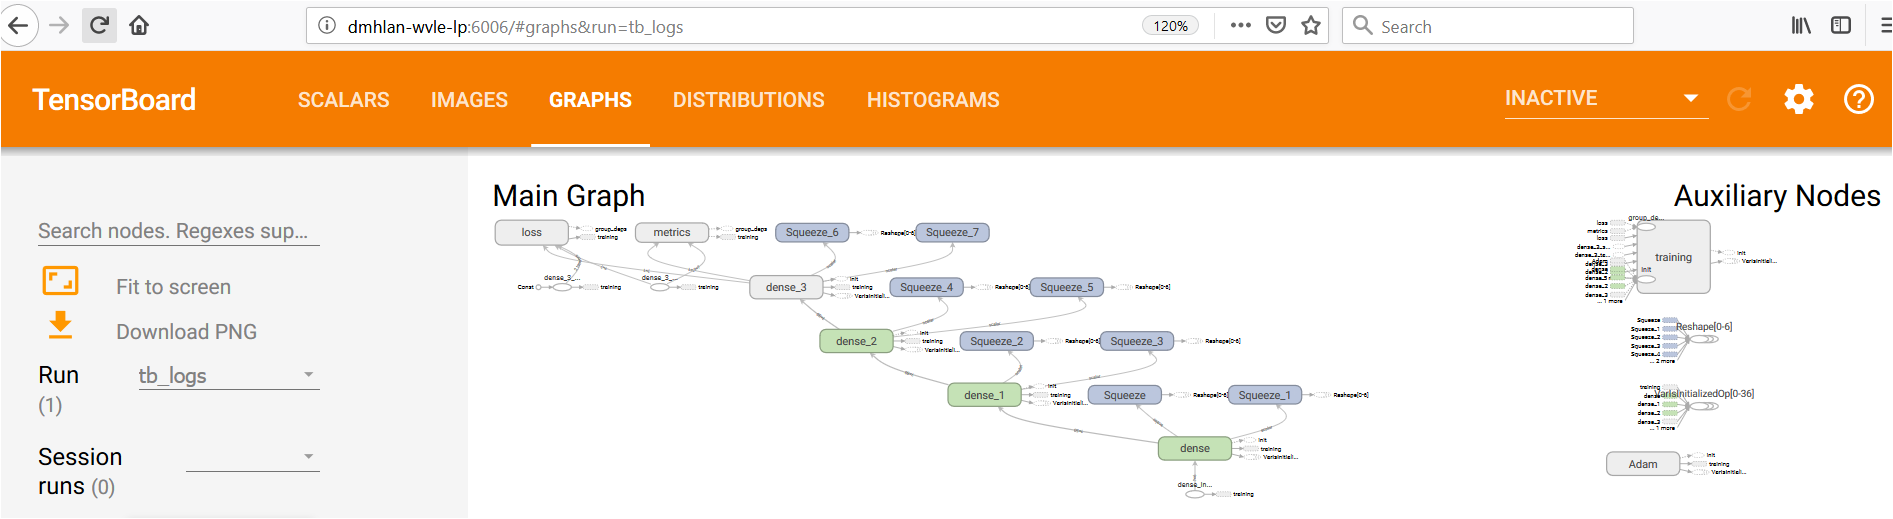
\includegraphics{main_graph.png}

\begin{figure}
\centering
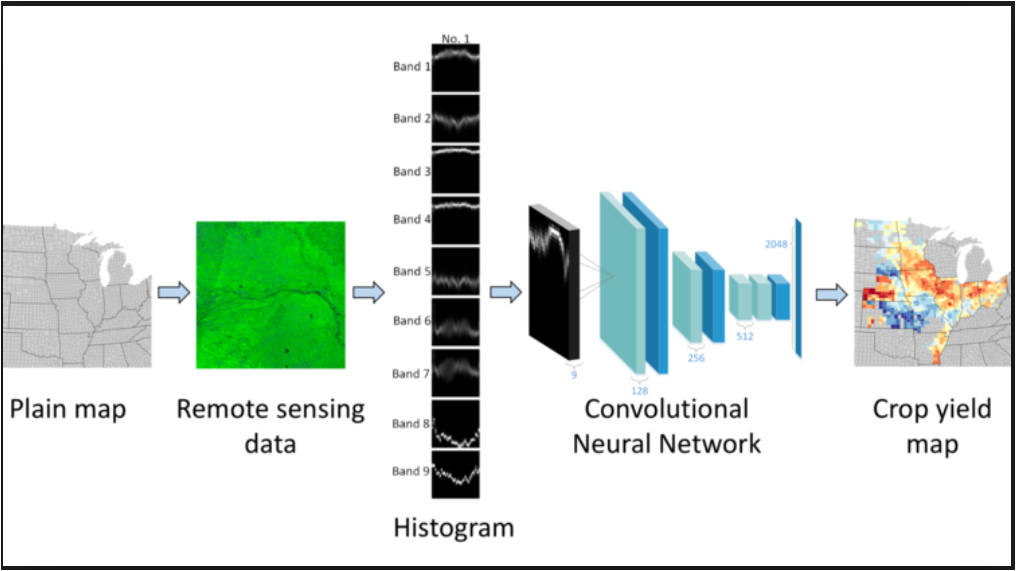
\includegraphics{analysis.png}
\caption{}
\end{figure}

Adopted from Stanford Data Science Institute

    \subsection{7. Hyperparameter Tuning applied to boost performance of
algorithm}\label{hyperparameter-tuning-applied-to-boost-performance-of-algorithm}

    \begin{Verbatim}[commandchars=\\\{\}]
{\color{incolor}In [{\color{incolor}44}]:} \PY{n}{model}\PY{o}{.}\PY{n}{compile}\PY{p}{(}\PY{n}{loss}\PY{o}{=}\PY{l+s+s1}{\PYZsq{}}\PY{l+s+s1}{binary\PYZus{}crossentropy}\PY{l+s+s1}{\PYZsq{}}\PY{p}{,} \PY{n}{optimizer}\PY{o}{=}\PY{l+s+s1}{\PYZsq{}}\PY{l+s+s1}{adam}\PY{l+s+s1}{\PYZsq{}}\PY{p}{,} \PY{n}{metrics}\PY{o}{=}\PY{p}{[}\PY{l+s+s1}{\PYZsq{}}\PY{l+s+s1}{accuracy}\PY{l+s+s1}{\PYZsq{}}\PY{p}{]}\PY{p}{)}
\end{Verbatim}


    \begin{Verbatim}[commandchars=\\\{\}]
{\color{incolor}In [{\color{incolor}45}]:} \PY{n}{tensorboard} \PY{o}{=} \PY{n}{tf}\PY{o}{.}\PY{n}{keras}\PY{o}{.}\PY{n}{callbacks}\PY{o}{.}\PY{n}{TensorBoard}\PY{p}{(}\PY{n}{log\PYZus{}dir}\PY{o}{=}\PY{l+s+s1}{\PYZsq{}}\PY{l+s+s1}{tb\PYZus{}logs}\PY{l+s+s1}{\PYZsq{}}\PY{p}{,} 
                                                      \PY{n}{histogram\PYZus{}freq}\PY{o}{=}\PY{l+m+mi}{1}\PY{p}{,}
                                                      \PY{n}{write\PYZus{}graph}\PY{o}{=}\PY{k+kc}{True}\PY{p}{,} 
                                                      \PY{n}{write\PYZus{}images}\PY{o}{=}\PY{k+kc}{True}\PY{p}{)}
\end{Verbatim}


    If you were to run the TensorBoard now, with \textbf{tensorboard
-\/-logdir=path/to/logs/directory}, \textbf{tensorboard
-\/-logdir="C:/Users/dmhlanga/Desktop/PythonProgrammingCUT/MachineLearningTechniques/Group\_One\_Assignment\_MSCDA605\_MachineLearning"},
you would see that in your given directory you get a folder named
`tb\_logs'. If you navigate to the ip address in your terminal, It will
take you to your TensorBoard, Then if you click graphs you will see your
graph.

\begin{figure}
\centering
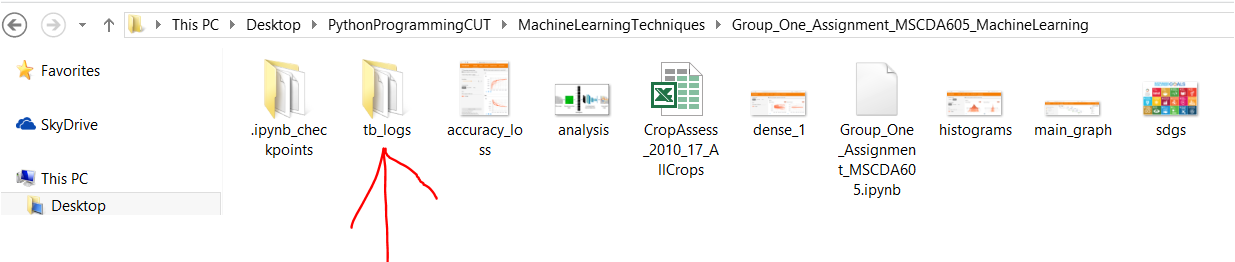
\includegraphics{tb_output.png}
\caption{}
\end{figure}

    \begin{Verbatim}[commandchars=\\\{\}]
{\color{incolor}In [{\color{incolor}46}]:} \PY{c+c1}{\PYZsh{}Here we are defining the name of the graph, scopes A, B and C.}
         \PY{k}{with} \PY{n}{tf}\PY{o}{.}\PY{n}{name\PYZus{}scope}\PY{p}{(}\PY{l+s+s2}{\PYZdq{}}\PY{l+s+s2}{MyOperationGroup}\PY{l+s+s2}{\PYZdq{}}\PY{p}{)}\PY{p}{:}
             \PY{k}{with} \PY{n}{tf}\PY{o}{.}\PY{n}{name\PYZus{}scope}\PY{p}{(}\PY{l+s+s2}{\PYZdq{}}\PY{l+s+s2}{Scope\PYZus{}A}\PY{l+s+s2}{\PYZdq{}}\PY{p}{)}\PY{p}{:}
                 \PY{n}{a} \PY{o}{=} \PY{n}{tf}\PY{o}{.}\PY{n}{add}\PY{p}{(}\PY{l+m+mi}{1}\PY{p}{,} \PY{l+m+mi}{2}\PY{p}{,} \PY{n}{name}\PY{o}{=}\PY{l+s+s2}{\PYZdq{}}\PY{l+s+s2}{Add\PYZus{}these\PYZus{}numbers}\PY{l+s+s2}{\PYZdq{}}\PY{p}{)}
                 \PY{n}{b} \PY{o}{=} \PY{n}{tf}\PY{o}{.}\PY{n}{multiply}\PY{p}{(}\PY{n}{a}\PY{p}{,} \PY{l+m+mi}{3}\PY{p}{)}
             \PY{k}{with} \PY{n}{tf}\PY{o}{.}\PY{n}{name\PYZus{}scope}\PY{p}{(}\PY{l+s+s2}{\PYZdq{}}\PY{l+s+s2}{Scope\PYZus{}B}\PY{l+s+s2}{\PYZdq{}}\PY{p}{)}\PY{p}{:}
                 \PY{n}{c} \PY{o}{=} \PY{n}{tf}\PY{o}{.}\PY{n}{add}\PY{p}{(}\PY{l+m+mi}{4}\PY{p}{,} \PY{l+m+mi}{5}\PY{p}{,} \PY{n}{name}\PY{o}{=}\PY{l+s+s2}{\PYZdq{}}\PY{l+s+s2}{And\PYZus{}These\PYZus{}ones}\PY{l+s+s2}{\PYZdq{}}\PY{p}{)}
                 \PY{n}{d} \PY{o}{=} \PY{n}{tf}\PY{o}{.}\PY{n}{multiply}\PY{p}{(}\PY{n}{c}\PY{p}{,} \PY{l+m+mi}{6}\PY{p}{,} \PY{n}{name}\PY{o}{=}\PY{l+s+s2}{\PYZdq{}}\PY{l+s+s2}{Multiply\PYZus{}these\PYZus{}numbers}\PY{l+s+s2}{\PYZdq{}}\PY{p}{)}
         
         \PY{k}{with} \PY{n}{tf}\PY{o}{.}\PY{n}{name\PYZus{}scope}\PY{p}{(}\PY{l+s+s2}{\PYZdq{}}\PY{l+s+s2}{Scope\PYZus{}C}\PY{l+s+s2}{\PYZdq{}}\PY{p}{)}\PY{p}{:}
             \PY{n}{e} \PY{o}{=} \PY{n}{tf}\PY{o}{.}\PY{n}{multiply}\PY{p}{(}\PY{l+m+mi}{4}\PY{p}{,} \PY{l+m+mi}{5}\PY{p}{,} \PY{n}{name}\PY{o}{=}\PY{l+s+s2}{\PYZdq{}}\PY{l+s+s2}{B\PYZus{}add}\PY{l+s+s2}{\PYZdq{}}\PY{p}{)}
             \PY{n}{f} \PY{o}{=} \PY{n}{tf}\PY{o}{.}\PY{n}{div}\PY{p}{(}\PY{n}{c}\PY{p}{,} \PY{l+m+mi}{6}\PY{p}{,} \PY{n}{name}\PY{o}{=}\PY{l+s+s2}{\PYZdq{}}\PY{l+s+s2}{B\PYZus{}mul}\PY{l+s+s2}{\PYZdq{}}\PY{p}{)}
         \PY{n}{g} \PY{o}{=} \PY{n}{tf}\PY{o}{.}\PY{n}{add}\PY{p}{(}\PY{n}{b}\PY{p}{,} \PY{n}{d}\PY{p}{)}
         \PY{n}{h} \PY{o}{=} \PY{n}{tf}\PY{o}{.}\PY{n}{multiply}\PY{p}{(}\PY{n}{g}\PY{p}{,} \PY{n}{f}\PY{p}{)}
\end{Verbatim}


    \begin{Verbatim}[commandchars=\\\{\}]
{\color{incolor}In [{\color{incolor}47}]:} \PY{n}{start\PYZus{}time} \PY{o}{=} \PY{n}{time}\PY{o}{.}\PY{n}{clock}\PY{p}{(}\PY{p}{)}
         \PY{n}{model}\PY{o}{.}\PY{n}{fit}\PY{p}{(}\PY{n}{X\PYZus{}train\PYZus{}std}\PY{p}{,} \PY{n}{y\PYZus{}train}\PY{p}{,} \PY{n}{epochs}\PY{o}{=}\PY{l+m+mi}{100}\PY{p}{,} \PY{n}{batch\PYZus{}size}\PY{o}{=}\PY{l+m+mi}{100}\PY{p}{,}\PY{n}{validation\PYZus{}split}\PY{o}{=}\PY{l+m+mf}{0.2}\PY{p}{,}\PY{n}{callbacks}\PY{o}{=}\PY{p}{[}\PY{n}{tensorboard}\PY{p}{]}\PY{p}{)}
         \PY{n+nb}{print}\PY{p}{(}\PY{n}{time}\PY{o}{.}\PY{n}{clock}\PY{p}{(}\PY{p}{)} \PY{o}{\PYZhy{}} \PY{n}{start\PYZus{}time}\PY{p}{,} \PY{l+s+s2}{\PYZdq{}}\PY{l+s+s2}{seconds}\PY{l+s+s2}{\PYZdq{}}\PY{p}{)}
\end{Verbatim}


    \begin{Verbatim}[commandchars=\\\{\}]
Train on 37398 samples, validate on 9350 samples
Epoch 1/100
37398/37398 [==============================] - 1s 32us/step - loss: 0.3765 - acc: 0.8679 - val\_loss: 0.3115 - val\_acc: 0.8878
Epoch 2/100
37398/37398 [==============================] - 1s 20us/step - loss: 0.3154 - acc: 0.8880 - val\_loss: 0.2969 - val\_acc: 0.8924
Epoch 3/100
37398/37398 [==============================] - 1s 19us/step - loss: 0.3037 - acc: 0.8913 - val\_loss: 0.2871 - val\_acc: 0.8973
Epoch 4/100
37398/37398 [==============================] - 1s 19us/step - loss: 0.2972 - acc: 0.8923 - val\_loss: 0.2821 - val\_acc: 0.8981
Epoch 5/100
37398/37398 [==============================] - 1s 20us/step - loss: 0.2917 - acc: 0.8937 - val\_loss: 0.2780 - val\_acc: 0.8980
Epoch 6/100
37398/37398 [==============================] - 1s 18us/step - loss: 0.2853 - acc: 0.8953 - val\_loss: 0.2693 - val\_acc: 0.8989
Epoch 7/100
37398/37398 [==============================] - 1s 17us/step - loss: 0.2740 - acc: 0.8988 - val\_loss: 0.2584 - val\_acc: 0.9050
Epoch 8/100
37398/37398 [==============================] - 1s 17us/step - loss: 0.2618 - acc: 0.9041 - val\_loss: 0.2471 - val\_acc: 0.9150
Epoch 9/100
37398/37398 [==============================] - 1s 18us/step - loss: 0.2523 - acc: 0.9092 - val\_loss: 0.2387 - val\_acc: 0.9158
Epoch 10/100
37398/37398 [==============================] - 1s 17us/step - loss: 0.2435 - acc: 0.9133 - val\_loss: 0.2347 - val\_acc: 0.9141
Epoch 11/100
37398/37398 [==============================] - 1s 19us/step - loss: 0.2374 - acc: 0.9151 - val\_loss: 0.2236 - val\_acc: 0.9227
Epoch 12/100
37398/37398 [==============================] - 1s 18us/step - loss: 0.2315 - acc: 0.9173 - val\_loss: 0.2217 - val\_acc: 0.9200
Epoch 13/100
37398/37398 [==============================] - 1s 17us/step - loss: 0.2268 - acc: 0.9194 - val\_loss: 0.2133 - val\_acc: 0.9308
Epoch 14/100
37398/37398 [==============================] - 1s 17us/step - loss: 0.2216 - acc: 0.9222 - val\_loss: 0.2109 - val\_acc: 0.9282
Epoch 15/100
37398/37398 [==============================] - 1s 21us/step - loss: 0.2179 - acc: 0.9238 - val\_loss: 0.2096 - val\_acc: 0.9258
Epoch 16/100
37398/37398 [==============================] - 1s 21us/step - loss: 0.2154 - acc: 0.9248 - val\_loss: 0.2032 - val\_acc: 0.9321
Epoch 17/100
37398/37398 [==============================] - 1s 21us/step - loss: 0.2110 - acc: 0.9258 - val\_loss: 0.2054 - val\_acc: 0.9276
Epoch 18/100
37398/37398 [==============================] - 1s 20us/step - loss: 0.2096 - acc: 0.9265 - val\_loss: 0.2002 - val\_acc: 0.9355
Epoch 19/100
37398/37398 [==============================] - 1s 25us/step - loss: 0.2069 - acc: 0.9278 - val\_loss: 0.2007 - val\_acc: 0.9318
Epoch 20/100
37398/37398 [==============================] - 1s 24us/step - loss: 0.2039 - acc: 0.9287 - val\_loss: 0.1962 - val\_acc: 0.9306
Epoch 21/100
37398/37398 [==============================] - 1s 24us/step - loss: 0.2020 - acc: 0.9293 - val\_loss: 0.1923 - val\_acc: 0.9361
Epoch 22/100
37398/37398 [==============================] - 1s 27us/step - loss: 0.1997 - acc: 0.9308 - val\_loss: 0.1910 - val\_acc: 0.9361
Epoch 23/100
37398/37398 [==============================] - 1s 24us/step - loss: 0.1981 - acc: 0.9306 - val\_loss: 0.1902 - val\_acc: 0.9354
Epoch 24/100
37398/37398 [==============================] - 1s 24us/step - loss: 0.1971 - acc: 0.9310 - val\_loss: 0.1910 - val\_acc: 0.9344
Epoch 25/100
37398/37398 [==============================] - 1s 22us/step - loss: 0.1950 - acc: 0.9326 - val\_loss: 0.1881 - val\_acc: 0.9383
Epoch 26/100
37398/37398 [==============================] - 1s 24us/step - loss: 0.1946 - acc: 0.9320 - val\_loss: 0.1943 - val\_acc: 0.9323
Epoch 27/100
37398/37398 [==============================] - 1s 24us/step - loss: 0.1930 - acc: 0.9321 - val\_loss: 0.1864 - val\_acc: 0.9379
Epoch 28/100
37398/37398 [==============================] - 1s 22us/step - loss: 0.1915 - acc: 0.9338 - val\_loss: 0.1901 - val\_acc: 0.9333
Epoch 29/100
37398/37398 [==============================] - 1s 21us/step - loss: 0.1899 - acc: 0.9337 - val\_loss: 0.1862 - val\_acc: 0.9370
Epoch 30/100
37398/37398 [==============================] - 1s 20us/step - loss: 0.1893 - acc: 0.9340 - val\_loss: 0.1850 - val\_acc: 0.9360
Epoch 31/100
37398/37398 [==============================] - 1s 19us/step - loss: 0.1883 - acc: 0.9341 - val\_loss: 0.1819 - val\_acc: 0.9390
Epoch 32/100
37398/37398 [==============================] - 1s 20us/step - loss: 0.1886 - acc: 0.9334 - val\_loss: 0.1886 - val\_acc: 0.9348
Epoch 33/100
37398/37398 [==============================] - 1s 20us/step - loss: 0.1867 - acc: 0.9345 - val\_loss: 0.1850 - val\_acc: 0.9356
Epoch 34/100
37398/37398 [==============================] - 1s 18us/step - loss: 0.1855 - acc: 0.9343 - val\_loss: 0.1823 - val\_acc: 0.9361
Epoch 35/100
37398/37398 [==============================] - 1s 28us/step - loss: 0.1864 - acc: 0.9339 - val\_loss: 0.1798 - val\_acc: 0.9393
Epoch 36/100
37398/37398 [==============================] - 1s 22us/step - loss: 0.1834 - acc: 0.9357 - val\_loss: 0.1786 - val\_acc: 0.9395
Epoch 37/100
37398/37398 [==============================] - 1s 21us/step - loss: 0.1834 - acc: 0.9353 - val\_loss: 0.1777 - val\_acc: 0.9407
Epoch 38/100
37398/37398 [==============================] - 1s 26us/step - loss: 0.1817 - acc: 0.9367 - val\_loss: 0.1756 - val\_acc: 0.9418
Epoch 39/100
37398/37398 [==============================] - 1s 25us/step - loss: 0.1817 - acc: 0.9359 - val\_loss: 0.1806 - val\_acc: 0.9383
Epoch 40/100
37398/37398 [==============================] - 1s 24us/step - loss: 0.1806 - acc: 0.9361 - val\_loss: 0.1750 - val\_acc: 0.9412
Epoch 41/100
37398/37398 [==============================] - 1s 22us/step - loss: 0.1807 - acc: 0.9358 - val\_loss: 0.1780 - val\_acc: 0.9399
Epoch 42/100
37398/37398 [==============================] - 1s 23us/step - loss: 0.1786 - acc: 0.9368 - val\_loss: 0.1747 - val\_acc: 0.9407
Epoch 43/100
37398/37398 [==============================] - 1s 27us/step - loss: 0.1778 - acc: 0.9375 - val\_loss: 0.1802 - val\_acc: 0.9379
Epoch 44/100
37398/37398 [==============================] - 1s 26us/step - loss: 0.1778 - acc: 0.9367 - val\_loss: 0.1729 - val\_acc: 0.9415
Epoch 45/100
37398/37398 [==============================] - 1s 21us/step - loss: 0.1773 - acc: 0.9376 - val\_loss: 0.1708 - val\_acc: 0.9420
Epoch 46/100
37398/37398 [==============================] - 1s 24us/step - loss: 0.1754 - acc: 0.9380 - val\_loss: 0.1780 - val\_acc: 0.9402
Epoch 47/100
37398/37398 [==============================] - 1s 22us/step - loss: 0.1757 - acc: 0.9380 - val\_loss: 0.1734 - val\_acc: 0.9426
Epoch 48/100
37398/37398 [==============================] - 1s 18us/step - loss: 0.1751 - acc: 0.9379 - val\_loss: 0.1709 - val\_acc: 0.9414
Epoch 49/100
37398/37398 [==============================] - 1s 18us/step - loss: 0.1739 - acc: 0.9386 - val\_loss: 0.1702 - val\_acc: 0.9425
Epoch 50/100
37398/37398 [==============================] - 1s 17us/step - loss: 0.1730 - acc: 0.9391 - val\_loss: 0.1691 - val\_acc: 0.9432
Epoch 51/100
37398/37398 [==============================] - 1s 18us/step - loss: 0.1740 - acc: 0.9380 - val\_loss: 0.1696 - val\_acc: 0.9419
Epoch 52/100
37398/37398 [==============================] - 1s 19us/step - loss: 0.1748 - acc: 0.9374 - val\_loss: 0.1643 - val\_acc: 0.9453
Epoch 53/100
37398/37398 [==============================] - 1s 18us/step - loss: 0.1712 - acc: 0.9394 - val\_loss: 0.1717 - val\_acc: 0.9385
Epoch 54/100
37398/37398 [==============================] - 1s 22us/step - loss: 0.1704 - acc: 0.9399 - val\_loss: 0.1630 - val\_acc: 0.9462
Epoch 55/100
37398/37398 [==============================] - 1s 21us/step - loss: 0.1693 - acc: 0.9402 - val\_loss: 0.1627 - val\_acc: 0.9462
Epoch 56/100
37398/37398 [==============================] - 1s 21us/step - loss: 0.1684 - acc: 0.9411 - val\_loss: 0.1726 - val\_acc: 0.9402
Epoch 57/100
37398/37398 [==============================] - 1s 18us/step - loss: 0.1678 - acc: 0.9411 - val\_loss: 0.1622 - val\_acc: 0.9451
Epoch 58/100
37398/37398 [==============================] - 1s 17us/step - loss: 0.1684 - acc: 0.9408 - val\_loss: 0.1654 - val\_acc: 0.9432
Epoch 59/100
37398/37398 [==============================] - 1s 20us/step - loss: 0.1665 - acc: 0.9416 - val\_loss: 0.1605 - val\_acc: 0.9471
Epoch 60/100
37398/37398 [==============================] - 1s 19us/step - loss: 0.1650 - acc: 0.9423 - val\_loss: 0.1599 - val\_acc: 0.9473
Epoch 61/100
37398/37398 [==============================] - 1s 19us/step - loss: 0.1663 - acc: 0.9414 - val\_loss: 0.1601 - val\_acc: 0.9453
Epoch 62/100
37398/37398 [==============================] - 1s 17us/step - loss: 0.1670 - acc: 0.9407 - val\_loss: 0.1649 - val\_acc: 0.9424
Epoch 63/100
37398/37398 [==============================] - 1s 18us/step - loss: 0.1636 - acc: 0.9422 - val\_loss: 0.1610 - val\_acc: 0.9437
Epoch 64/100
37398/37398 [==============================] - 1s 17us/step - loss: 0.1636 - acc: 0.9415 - val\_loss: 0.1582 - val\_acc: 0.9495
Epoch 65/100
37398/37398 [==============================] - 1s 19us/step - loss: 0.1636 - acc: 0.9424 - val\_loss: 0.1568 - val\_acc: 0.9458
Epoch 66/100
37398/37398 [==============================] - 1s 18us/step - loss: 0.1613 - acc: 0.9423 - val\_loss: 0.1566 - val\_acc: 0.9490
Epoch 67/100
37398/37398 [==============================] - 1s 17us/step - loss: 0.1596 - acc: 0.9429 - val\_loss: 0.1595 - val\_acc: 0.9436
Epoch 68/100
37398/37398 [==============================] - 1s 20us/step - loss: 0.1598 - acc: 0.9433 - val\_loss: 0.1541 - val\_acc: 0.9462
Epoch 69/100
37398/37398 [==============================] - 1s 19us/step - loss: 0.1594 - acc: 0.9424 - val\_loss: 0.1533 - val\_acc: 0.9464
Epoch 70/100
37398/37398 [==============================] - 1s 18us/step - loss: 0.1568 - acc: 0.9439 - val\_loss: 0.1490 - val\_acc: 0.9478
Epoch 71/100
37398/37398 [==============================] - 1s 17us/step - loss: 0.1524 - acc: 0.9451 - val\_loss: 0.1466 - val\_acc: 0.9491
Epoch 72/100
37398/37398 [==============================] - 1s 20us/step - loss: 0.1518 - acc: 0.9453 - val\_loss: 0.1522 - val\_acc: 0.9439
Epoch 73/100
37398/37398 [==============================] - 1s 18us/step - loss: 0.1494 - acc: 0.9456 - val\_loss: 0.1399 - val\_acc: 0.9516
Epoch 74/100
37398/37398 [==============================] - 1s 17us/step - loss: 0.1449 - acc: 0.9470 - val\_loss: 0.1409 - val\_acc: 0.9486
Epoch 75/100
37398/37398 [==============================] - 1s 17us/step - loss: 0.1427 - acc: 0.9477 - val\_loss: 0.1472 - val\_acc: 0.9468
Epoch 76/100
37398/37398 [==============================] - 1s 18us/step - loss: 0.1370 - acc: 0.9492 - val\_loss: 0.1302 - val\_acc: 0.9526
Epoch 77/100
37398/37398 [==============================] - 1s 19us/step - loss: 0.1371 - acc: 0.9498 - val\_loss: 0.1270 - val\_acc: 0.9547
Epoch 78/100
37398/37398 [==============================] - 1s 20us/step - loss: 0.1320 - acc: 0.9510 - val\_loss: 0.1248 - val\_acc: 0.9540
Epoch 79/100
37398/37398 [==============================] - 1s 19us/step - loss: 0.1277 - acc: 0.9536 - val\_loss: 0.1230 - val\_acc: 0.9539
Epoch 80/100
37398/37398 [==============================] - 1s 19us/step - loss: 0.1252 - acc: 0.9533 - val\_loss: 0.1172 - val\_acc: 0.9563
Epoch 81/100
37398/37398 [==============================] - 1s 18us/step - loss: 0.1255 - acc: 0.9534 - val\_loss: 0.1163 - val\_acc: 0.9583
Epoch 82/100
37398/37398 [==============================] - 1s 17us/step - loss: 0.1232 - acc: 0.9542 - val\_loss: 0.1144 - val\_acc: 0.9583
Epoch 83/100
37398/37398 [==============================] - 1s 18us/step - loss: 0.1203 - acc: 0.9560 - val\_loss: 0.1162 - val\_acc: 0.9590
Epoch 84/100
37398/37398 [==============================] - 1s 21us/step - loss: 0.1195 - acc: 0.9555 - val\_loss: 0.1235 - val\_acc: 0.9545
Epoch 85/100
37398/37398 [==============================] - 1s 19us/step - loss: 0.1174 - acc: 0.9572 - val\_loss: 0.1369 - val\_acc: 0.9506
Epoch 86/100
37398/37398 [==============================] - 1s 18us/step - loss: 0.1163 - acc: 0.9571 - val\_loss: 0.1075 - val\_acc: 0.9590
Epoch 87/100
37398/37398 [==============================] - 1s 21us/step - loss: 0.1139 - acc: 0.9571 - val\_loss: 0.1140 - val\_acc: 0.9567
Epoch 88/100
37398/37398 [==============================] - 1s 18us/step - loss: 0.1159 - acc: 0.9566 - val\_loss: 0.1053 - val\_acc: 0.9618
Epoch 89/100
37398/37398 [==============================] - 1s 23us/step - loss: 0.1106 - acc: 0.9586 - val\_loss: 0.1018 - val\_acc: 0.9626
Epoch 90/100
37398/37398 [==============================] - 1s 22us/step - loss: 0.1120 - acc: 0.9587 - val\_loss: 0.1019 - val\_acc: 0.9615
Epoch 91/100
37398/37398 [==============================] - 1s 20us/step - loss: 0.1127 - acc: 0.9581 - val\_loss: 0.1118 - val\_acc: 0.9570
Epoch 92/100
37398/37398 [==============================] - 1s 18us/step - loss: 0.1113 - acc: 0.9584 - val\_loss: 0.1075 - val\_acc: 0.9613
Epoch 93/100
37398/37398 [==============================] - 1s 18us/step - loss: 0.1084 - acc: 0.9596 - val\_loss: 0.1108 - val\_acc: 0.9607
Epoch 94/100
37398/37398 [==============================] - 1s 18us/step - loss: 0.1074 - acc: 0.9596 - val\_loss: 0.1376 - val\_acc: 0.9530
Epoch 95/100
37398/37398 [==============================] - 1s 20us/step - loss: 0.1065 - acc: 0.9594 - val\_loss: 0.1024 - val\_acc: 0.9670
Epoch 96/100
37398/37398 [==============================] - 1s 19us/step - loss: 0.1049 - acc: 0.9609 - val\_loss: 0.1053 - val\_acc: 0.9616
Epoch 97/100
37398/37398 [==============================] - 1s 19us/step - loss: 0.1082 - acc: 0.9595 - val\_loss: 0.1228 - val\_acc: 0.9523
Epoch 98/100
37398/37398 [==============================] - 1s 19us/step - loss: 0.1045 - acc: 0.9610 - val\_loss: 0.1368 - val\_acc: 0.9466
Epoch 99/100
37398/37398 [==============================] - 1s 19us/step - loss: 0.1020 - acc: 0.9617 - val\_loss: 0.1057 - val\_acc: 0.9628
Epoch 100/100
37398/37398 [==============================] - 1s 20us/step - loss: 0.1033 - acc: 0.9615 - val\_loss: 0.0915 - val\_acc: 0.9656
86.33417096602028 seconds

    \end{Verbatim}

    \subsection{8. Performance Metrics of the Machine learning / Deep
learning
algorithm}\label{performance-metrics-of-the-machine-learning-deep-learning-algorithm}

    \subsubsection{TensorBoard outputs}\label{tensorboard-outputs}

Accuracy\_Loss

\begin{figure}
\centering
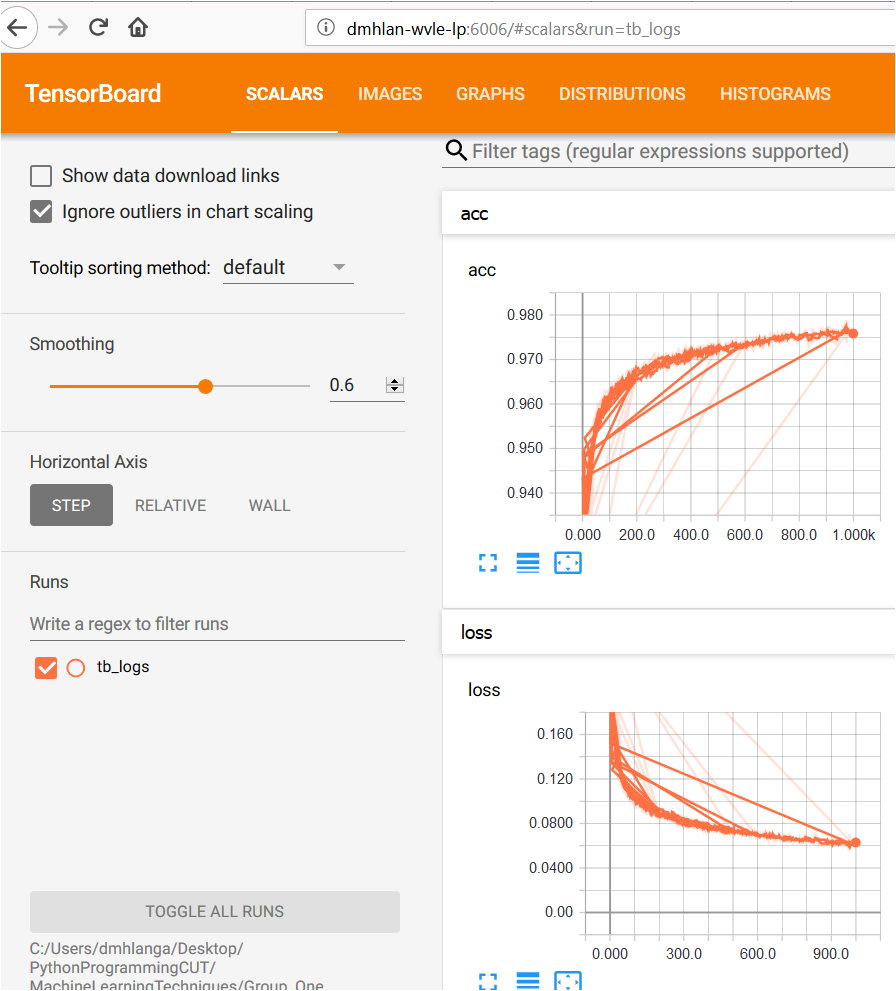
\includegraphics{accuracy_loss.png}
\caption{}
\end{figure}

Dense step

\begin{figure}
\centering
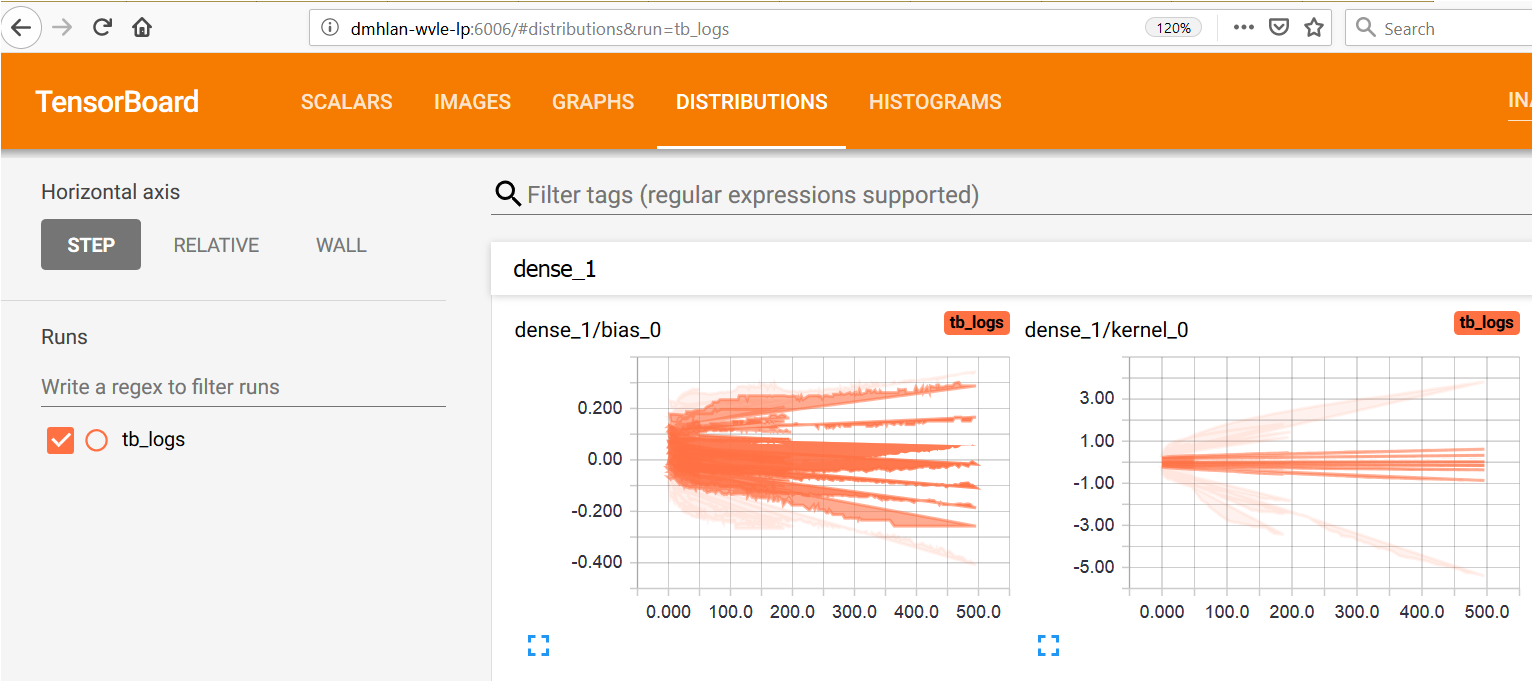
\includegraphics{dense_1.png}
\caption{}
\end{figure}

Histograms

\begin{figure}
\centering
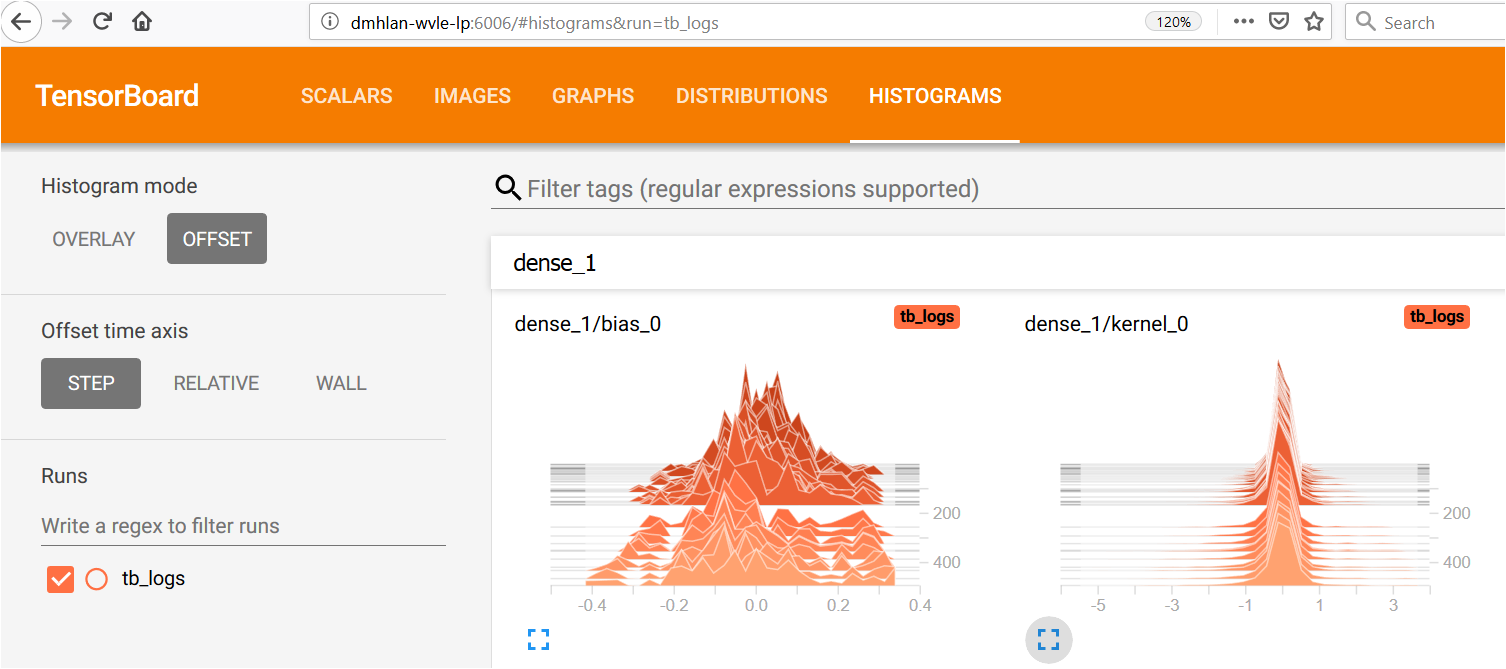
\includegraphics{histograms.png}
\caption{}
\end{figure}

    \begin{Verbatim}[commandchars=\\\{\}]
{\color{incolor}In [{\color{incolor}48}]:} \PY{n}{scores} \PY{o}{=} \PY{n}{model}\PY{o}{.}\PY{n}{evaluate}\PY{p}{(}\PY{n}{X\PYZus{}test\PYZus{}std}\PY{p}{,} \PY{n}{y\PYZus{}test}\PY{p}{)}
         \PY{n+nb}{print}\PY{p}{(}\PY{l+s+s2}{\PYZdq{}}\PY{l+s+si}{\PYZpc{}s}\PY{l+s+s2}{: }\PY{l+s+si}{\PYZpc{}.2f}\PY{l+s+si}{\PYZpc{}\PYZpc{}}\PY{l+s+s2}{\PYZdq{}} \PY{o}{\PYZpc{}} \PY{p}{(}\PY{n}{model}\PY{o}{.}\PY{n}{metrics\PYZus{}names}\PY{p}{[}\PY{l+m+mi}{1}\PY{p}{]}\PY{p}{,} \PY{n}{scores}\PY{p}{[}\PY{l+m+mi}{1}\PY{p}{]}\PY{o}{*}\PY{l+m+mi}{100}\PY{p}{)}\PY{p}{)}
\end{Verbatim}


    \begin{Verbatim}[commandchars=\\\{\}]
11688/11688 [==============================] - 0s 34us/step
acc: 92.93\%

    \end{Verbatim}

    \begin{Verbatim}[commandchars=\\\{\}]
{\color{incolor}In [{\color{incolor}49}]:} \PY{k+kn}{import} \PY{n+nn}{seaborn} \PY{k}{as} \PY{n+nn}{sns}
         \PY{k+kn}{from} \PY{n+nn}{datetime} \PY{k}{import} \PY{n}{datetime}
         \PY{k+kn}{from} \PY{n+nn}{matplotlib}\PY{n+nn}{.}\PY{n+nn}{colors} \PY{k}{import} \PY{n}{ListedColormap}
         \PY{k+kn}{from} \PY{n+nn}{sklearn}\PY{n+nn}{.}\PY{n+nn}{datasets} \PY{k}{import} \PY{n}{make\PYZus{}classification}\PY{p}{,} \PY{n}{make\PYZus{}moons}\PY{p}{,} \PY{n}{make\PYZus{}circles}
         \PY{k+kn}{from} \PY{n+nn}{sklearn}\PY{n+nn}{.}\PY{n+nn}{metrics} \PY{k}{import} \PY{n}{confusion\PYZus{}matrix}\PY{p}{,} \PY{n}{classification\PYZus{}report}\PY{p}{,} \PY{n}{mean\PYZus{}squared\PYZus{}error}\PY{p}{,} \PY{n}{mean\PYZus{}absolute\PYZus{}error}\PY{p}{,} \PY{n}{r2\PYZus{}score}
         \PY{k+kn}{from} \PY{n+nn}{sklearn}\PY{n+nn}{.}\PY{n+nn}{linear\PYZus{}model} \PY{k}{import} \PY{n}{LogisticRegression}
         \PY{k+kn}{from} \PY{n+nn}{sklearn}\PY{n+nn}{.}\PY{n+nn}{utils} \PY{k}{import} \PY{n}{shuffle}
         
         \PY{k+kn}{from} \PY{n+nn}{sklearn}\PY{n+nn}{.}\PY{n+nn}{preprocessing} \PY{k}{import} \PY{n}{StandardScaler}\PY{p}{,} \PY{n}{LabelEncoder}\PY{p}{,} \PY{n}{OneHotEncoder}\PY{p}{,} \PY{n}{MinMaxScaler}
         \PY{k+kn}{from} \PY{n+nn}{sklearn}\PY{n+nn}{.}\PY{n+nn}{model\PYZus{}selection} \PY{k}{import} \PY{n}{train\PYZus{}test\PYZus{}split}\PY{p}{,} \PY{n}{cross\PYZus{}val\PYZus{}score}\PY{p}{,} \PY{n}{StratifiedKFold}\PY{p}{,} \PY{n}{KFold}
\end{Verbatim}


    \begin{Verbatim}[commandchars=\\\{\}]
{\color{incolor}In [{\color{incolor}50}]:} \PY{k}{def} \PY{n+nf}{plot\PYZus{}confusion\PYZus{}matrix}\PY{p}{(}\PY{n}{model}\PY{p}{,} \PY{n}{X}\PY{p}{,} \PY{n}{y}\PY{p}{)}\PY{p}{:}
             \PY{n}{y\PYZus{}pred} \PY{o}{=} \PY{n}{model}\PY{o}{.}\PY{n}{predict\PYZus{}classes}\PY{p}{(}\PY{n}{X}\PY{p}{,} \PY{n}{verbose}\PY{o}{=}\PY{l+m+mi}{0}\PY{p}{)}
             \PY{n}{plt}\PY{o}{.}\PY{n}{figure}\PY{p}{(}\PY{n}{figsize}\PY{o}{=}\PY{p}{(}\PY{l+m+mi}{8}\PY{p}{,} \PY{l+m+mi}{6}\PY{p}{)}\PY{p}{)}
             \PY{n}{sns}\PY{o}{.}\PY{n}{heatmap}\PY{p}{(}\PY{n}{pd}\PY{o}{.}\PY{n}{DataFrame}\PY{p}{(}\PY{n}{confusion\PYZus{}matrix}\PY{p}{(}\PY{n}{y}\PY{p}{,} \PY{n}{y\PYZus{}pred}\PY{p}{)}\PY{p}{)}\PY{p}{,} \PY{n}{annot}\PY{o}{=}\PY{k+kc}{True}\PY{p}{,} \PY{n}{fmt}\PY{o}{=}\PY{l+s+s1}{\PYZsq{}}\PY{l+s+s1}{d}\PY{l+s+s1}{\PYZsq{}}\PY{p}{,} \PY{n}{cmap}\PY{o}{=}\PY{l+s+s1}{\PYZsq{}}\PY{l+s+s1}{YlGnBu}\PY{l+s+s1}{\PYZsq{}}\PY{p}{,} \PY{n}{alpha}\PY{o}{=}\PY{l+m+mf}{0.8}\PY{p}{,} \PY{n}{vmin}\PY{o}{=}\PY{l+m+mi}{0}\PY{p}{)}
\end{Verbatim}


    \begin{Verbatim}[commandchars=\\\{\}]
{\color{incolor}In [{\color{incolor}51}]:} \PY{n}{y\PYZus{}pred} \PY{o}{=} \PY{n}{model}\PY{o}{.}\PY{n}{predict\PYZus{}classes}\PY{p}{(}\PY{n}{X}\PY{p}{,} \PY{n}{verbose}\PY{o}{=}\PY{l+m+mi}{0}\PY{p}{)}
         \PY{n+nb}{print}\PY{p}{(}\PY{n}{classification\PYZus{}report}\PY{p}{(}\PY{n}{Y}\PY{p}{,} \PY{n}{y\PYZus{}pred}\PY{p}{)}\PY{p}{)}
\end{Verbatim}


    \begin{Verbatim}[commandchars=\\\{\}]
             precision    recall  f1-score   support

        0.0       1.00      0.10      0.18     50640
        1.0       0.15      1.00      0.25      7796

avg / total       0.89      0.22      0.19     58436


    \end{Verbatim}

    \begin{Verbatim}[commandchars=\\\{\}]
{\color{incolor}In [{\color{incolor}52}]:} \PY{n}{plot\PYZus{}confusion\PYZus{}matrix}\PY{p}{(}\PY{n}{model}\PY{p}{,} \PY{n}{X}\PY{p}{,} \PY{n}{Y}\PY{p}{)}
\end{Verbatim}


    \begin{center}
    \adjustimage{max size={0.9\linewidth}{0.9\paperheight}}{output_66_0.png}
    \end{center}
    { \hspace*{\fill} \\}
    
    \subsection{9. The analytics outcome (What insights can you provide from
this
data)}\label{the-analytics-outcome-what-insights-can-you-provide-from-this-data}

The model as shown by the metrics of about 92.86\% accuracy is able to
predict precicely the expected crop yields in the future harvests. A
classification report below shows that Precision is averaged at 0.88,
Recall of 0.13 and f1-score of 0.03.

\begin{longtable}[]{@{}l@{}}
\toprule
0.0\tabularnewline
1.0\tabularnewline
Avg/total\tabularnewline
\bottomrule
\end{longtable}

    \subsection{Linear regression}\label{linear-regression}

Using linear regression to predict the yeild given area, production,
crop, sector and wardpcode

    \begin{Verbatim}[commandchars=\\\{\}]
{\color{incolor}In [{\color{incolor}53}]:} \PY{k+kn}{from} \PY{n+nn}{sklearn} \PY{k}{import} \PY{n}{linear\PYZus{}model}
\end{Verbatim}


    \begin{Verbatim}[commandchars=\\\{\}]
{\color{incolor}In [{\color{incolor}54}]:} \PY{n}{reg} \PY{o}{=}\PY{n}{linear\PYZus{}model}\PY{o}{.}\PY{n}{LinearRegression}\PY{p}{(}\PY{p}{)}
\end{Verbatim}


    \begin{Verbatim}[commandchars=\\\{\}]
{\color{incolor}In [{\color{incolor}55}]:} \PY{n}{df}\PY{o}{.}\PY{n}{head}\PY{p}{(}\PY{p}{)}
\end{Verbatim}


\begin{Verbatim}[commandchars=\\\{\}]
{\color{outcolor}Out[{\color{outcolor}55}]:}           Area          Pdn  data\_Crop  data\_Sector  data\_WardPCode  \textbackslash{}
         0   368.106659     0.000000          0            5            1017   
         1  3692.266846  5894.784668          0            4             148   
         2  1838.549927  1044.947510          0            2            1462   
         4     9.450000     1.228000          0            1             918   
         5  1628.263306  2673.965332          0            2             766   
         
            Final\_yeild       profit  
         0     0.000000     0.000000  
         1  1596.521854 -4298.262814  
         2   568.354189  -476.593320  
         4   129.947096   128.719096  
         5  1642.219186 -1031.746146  
\end{Verbatim}
            
    Selecting feature space and feature label space, in this case our
features are

\begin{itemize}
\tightlist
\item
  area, production, crop, sector and wardpcode
\end{itemize}

    \begin{Verbatim}[commandchars=\\\{\}]
{\color{incolor}In [{\color{incolor}56}]:} \PY{n}{reg}\PY{o}{.}\PY{n}{fit}\PY{p}{(}\PY{n}{df}\PY{p}{[}\PY{p}{[}\PY{l+s+s1}{\PYZsq{}}\PY{l+s+s1}{Area}\PY{l+s+s1}{\PYZsq{}}\PY{p}{,}\PY{l+s+s1}{\PYZsq{}}\PY{l+s+s1}{Pdn}\PY{l+s+s1}{\PYZsq{}}\PY{p}{,}\PY{l+s+s1}{\PYZsq{}}\PY{l+s+s1}{data\PYZus{}Crop}\PY{l+s+s1}{\PYZsq{}}\PY{p}{,}\PY{l+s+s1}{\PYZsq{}}\PY{l+s+s1}{data\PYZus{}Sector}\PY{l+s+s1}{\PYZsq{}}\PY{p}{,}\PY{l+s+s1}{\PYZsq{}}\PY{l+s+s1}{data\PYZus{}WardPCode}\PY{l+s+s1}{\PYZsq{}}\PY{p}{]}\PY{p}{]}\PY{p}{,}\PY{n}{df}\PY{o}{.}\PY{n}{Final\PYZus{}yeild}\PY{p}{)}
\end{Verbatim}


\begin{Verbatim}[commandchars=\\\{\}]
{\color{outcolor}Out[{\color{outcolor}56}]:} LinearRegression(copy\_X=True, fit\_intercept=True, n\_jobs=1, normalize=False)
\end{Verbatim}
            
    \paragraph{Coefficients}\label{coefficients}

    \begin{Verbatim}[commandchars=\\\{\}]
{\color{incolor}In [{\color{incolor}57}]:} \PY{n}{reg}\PY{o}{.}\PY{n}{coef\PYZus{}}
\end{Verbatim}


\begin{Verbatim}[commandchars=\\\{\}]
{\color{outcolor}Out[{\color{outcolor}57}]:} array([-8.19160802e-02,  5.63965067e-01, -2.05036282e+01, -1.09615580e+02,
                -6.38206406e-01])
\end{Verbatim}
            
    \paragraph{Intercept}\label{intercept}

    \begin{Verbatim}[commandchars=\\\{\}]
{\color{incolor}In [{\color{incolor}58}]:} \PY{n}{reg}\PY{o}{.}\PY{n}{intercept\PYZus{}}
\end{Verbatim}


\begin{Verbatim}[commandchars=\\\{\}]
{\color{outcolor}Out[{\color{outcolor}58}]:} 1760.9049658388662
\end{Verbatim}
            
    \paragraph{Predicting yeild given
features}\label{predicting-yeild-given-features}

    \begin{Verbatim}[commandchars=\\\{\}]
{\color{incolor}In [{\color{incolor}59}]:} \PY{n}{reg}\PY{o}{.}\PY{n}{predict}\PY{p}{(}\PY{p}{[}\PY{p}{[}\PY{l+m+mi}{4000}\PY{p}{,}\PY{l+m+mf}{1.33}\PY{p}{,}\PY{l+m+mi}{0}\PY{p}{,}\PY{l+m+mi}{5}\PY{p}{,}\PY{l+m+mi}{1017}\PY{p}{]}\PY{p}{]}\PY{p}{)}
\end{Verbatim}


\begin{Verbatim}[commandchars=\\\{\}]
{\color{outcolor}Out[{\color{outcolor}59}]:} array([236.85690258])
\end{Verbatim}
            
    \subsection{10. Conclusion and Remarks}\label{conclusion-and-remarks}

We can conclude that after tweeking the variable hyperparameters upwards
or downwards like epochs=200, batch\_size=100,and validation\_split=0.2
our predicted accuracy improves. The top six classified crops showed
differences in crop yields per each class. Our Zimbabwean prediction for
crop yield need to improve by installation of sensors in the cropping
fields, like an example from Stanford Data Science Institute, wose
objective is to understand worldwide crop yield which is central to
suistable development. It can help achieve zero hunger, which is among
the top of UN Sustainable Development Goals for the year of 2030. In the
project, Stanford Data Science Institute introduce a scalable, accurate,
and inexpensive method to predict crop yield using publicly available
remote sensing data and machine learning. Their deep learning approach
can predict crop yield with high spatial resolution (county-level)
several months before harvest, using only globally available covariates.
They believe their solution can potentially help making informed
planting decisions, setting appropriate food reserve level, identifying
low-yield regions and improving risk management of crop-related
derivatives.

    \subsection{References}\label{references}

\begin{itemize}
\tightlist
\item
  Central Statistical Office (Zimbabwe, www.zimstat.co.zw/
\item
  http://sustain.stanford.edu/crop-yield-analysis/
\item
  https://dataskeptic.com/blog/episodes/2017/convolutional-neural-networks;
\item
  https://www.tensorflow.org/;
\item
  https://www.datascience.com;
\item
  https://colab.research.google.com/;
\item
  https://medium.com/;
\item
  https://codeburst.io/;
\item
  http://ufldl.stanford.edu
\end{itemize}


    % Add a bibliography block to the postdoc
    
    
    
    \end{document}
